\documentclass{formato/UNIR}

%--- Parametros de entrada ---%
\titulo{Diseño de un asistente institucional, RAG e integración de herramientas}
\autor{Nuria Iglesias Traviesa}
\director{David Jiménez Cabello}
\fecha{22/04/2026}
\ciudad{Valencia}
\universidad{Universidad Internacional de la Rioja (UNIR)}
\escuela{Escuela Superior de Ingeniería y Tecnología}
\master{Master universitario en Inteligencia Artificial}
\tipoTesis{Trabajo Fin de Máster}

\keywords{Large Language Models, Retrieval-Augmented Generation, Hybrid Retrieval, Reranking, Tool Use, Institutional Assistant}
\keywordsEs{Modelos de lenguaje de gran tamaño, Retrieval-Augmented Generation, Recuperación híbrida, Reranking, Uso de herramientas, Asistente institucional}


%--- Archivo de configuracion global ---%
\input{formato/conf}

%---  Compilacion rapida ---%
% Para ahorrar tiempo de compilacion, comentar las secciones que no se quieran compilar
% Carácter % en frente de la sección.
\includeonly{
  contenido/TFM-00_Abstract,
  contenido/TFM-01_Introduccion,
  contenido/TFM-02_EstadoDelArte,
  contenido/TFM-03_Objetivos_y_Metodologia,
  contenido/TFM-04_Fundamentos_Tecnologicos,
  contenido/TFM-09_Resultados,
  contenido/TFM-10_Bibliografia,
  contenido/TFM-11_Apendice_1,
%   contenido/TFM-11_Apendice_2 
}

%---------------------------------------------%
%           Inicio del documento
%---------------------------------------------%
\begin{document}
    %--- Paginas iniciales: portada,abstract,índice,lista de figuras y lista de tablas ---%. 
    \frontmatter
    \pagestyle{frontmatter}
        \maketitle          % Portada
        \tableofcontents    % Índice
        \clearpage
        \begin{abstract}[Resumen]
Este Trabajo de Fin de Máster presenta el diseño, implementación y evaluación de un asistente institucional basado en \textit{Retrieval-Augmented Generation} (RAG) e integración de herramientas. La arquitectura propuesta combina recuperación documental sobre un corpus de fuentes institucionales, mejora del \textit{ranking} de evidencias mediante recuperación híbrida y \textit{reranking}, orquestación del flujo de interacción basado en agente y generación y envío supervisado de correos electrónicos.

El sistema se evalúa mediante un \textit{ablation study} con cuatro variantes progresivas sobre un dataset de 71 preguntas anotadas manualmente sobre documentación pública de UNIR, analizando el impacto de cada componente sobre métricas de recuperación (Hit@1, Hit@3, MRR) y de generación (Fact-Coverage, ROUGE-L, BERTScore).

Los resultados muestran que la recuperación híbrida y el \textit{reranking} incrementan la cobertura factual un 35,5\,\% respecto al \textit{baseline} (de 0.389 a 0.527) y mejoran la cobertura en el top-3 (Hit@3 = 0.918). El orquestador aporta valor en términos de control del flujo, abstención ante preguntas no respondibles y activación de herramientas accionables, con una calidad semántica equivalente a la variante determinista (BERTScore 0.648 frente a 0.656). En conjunto, los resultados sugieren la utilidad de una arquitectura modular, trazable y supervisada para asistentes institucionales privados.

\textbf{Palabras clave:} Modelos de lenguaje de gran tamaño, Retrieval-Augmented Generation, recuperación híbrida, reranking, orquestación, uso de herramientas, asistente institucional.
\end{abstract}


\pagebreak
%Ingles
\begin{abstract}[Abstract]
This Master's Thesis presents the design, implementation and evaluation of an institutional assistant based on Retrieval-Augmented Generation (RAG) and tool integration. The proposed architecture combines document retrieval over an institutional corpus, evidence ranking improvement through hybrid retrieval and reranking, agent-based interaction flow orchestration, and supervised generation and sending of emails.

The system is evaluated through a four-variant ablation study on a manually annotated dataset of 71 questions over public UNIR documentation, measuring the impact of each component on retrieval metrics (Hit@1, Hit@3, MRR) and generation metrics (Fact-Coverage, ROUGE-L, BERTScore).

Results show that hybrid retrieval and reranking improve fact coverage by 35.5\% over the baseline (from 0.389 to 0.527) and increase top-3 coverage (Hit@3 = 0.918). The orchestrator contributes flow control, abstention on unanswerable questions and activation of actionable tools, with semantic quality equivalent to the deterministic variant (BERTScore 0.648 vs 0.656). Overall, the results suggest the usefulness of a modular, traceable and supervised architecture for private institutional assistants.

\textbf{Keywords:} Large Language Models, Retrieval-Augmented Generation, hybrid retrieval, reranking, orchestration, tool use, institutional assistant.
\end{abstract}  %Abtract
        \listoffigures      % Índice de imagenes
        \listoftables       % Índice de tablas
    
    %---    Cuerpo ---% 
    \mainmatter
    \pagestyle{mainmatter}
        %Incluir aqui todos los capitulos (carpeta contenido)
    	\chapter{Introducción}\label{chap:introduccion}

En este primer capítulo se presenta el sistema de agentes con integración de herramientas orientadas a la realización de acciones útiles para el usuario, así como la propuesta de mejora del componente RAG. 
Asimismo, se describen la motivación y el contexto del trabajo, el planteamiento general de la solución, los objetivos a grandes rasgos y la estructura del documento.

\section{Motivación}

La motivación principal de este trabajo surge de la necesidad de explorar cómo diseñar un asistente institucional que combine consulta documental y capacidad de realizar acciones. 
Frente a enfoques centrados exclusivamente en la generación de respuestas, se parte de la idea de que un asistente útil en un entorno institucional debe ser capaz no solo de informar, sino también de ayudar a materializar el siguiente paso de manera controlada y supervisada por el ser humano.

Esta necesidad resulta especialmente visible en el ámbito universitario, donde parte de la información relevante para el estudiante se encuentra dispersa en normativas, páginas web, documentos administrativos o guías internas cuya consulta no siempre es sencilla. 
Cuestiones relacionadas con trámites, prácticas, horarios o becas pueden generar dudas incluso cuando la información existe, simplemente porque no resulta fácilmente accesible o comprensible. 
En este contexto, disponer de un asistente capaz de responder de forma clara, fundamentada y contextualizada puede suponer una mejora significativa en la experiencia del usuario, especialmente si se tiene en cuenta que muchas instituciones universitarias todavía no cuentan con herramientas conversacionales suficientemente útiles, especializadas o integradas para este tipo de consultas.

A ello se añade una segunda motivación de carácter investigador. 
En sistemas basados en \textit{Retrieval-Augmented Generation} (RAG), la calidad de la recuperación documental condiciona directamente la calidad de las respuestas generadas. 
Por este motivo, resulta de interés analizar si una mejora concreta del componente de recuperación, basada en estrategias de recuperación híbrida y \textit{reranking} \parencite{nogueira2020monot5}, puede traducirse en una mejora observable en las respuestas y en la utilidad general del asistente. 
De este modo, el trabajo no solo responde a una necesidad práctica de desarrollo, sino también a una pregunta aplicada de investigación sobre el impacto real de optimizar el \textit{retrieval} en asistentes institucionales.

\section{Planteamiento del trabajo}\label{sec:planteamiento_solucion}

Se propone el desarrollo de un asistente conversacional institucional privado que permita consultar documentación interna, ofrecer respuestas fundamentadas y apoyar acciones útiles para el usuario dentro de un entorno controlado.

Esta propuesta no aspira únicamente a construir un sistema conversacional más, sino a desarrollar una solución capaz de combinar acceso a conocimiento documental, razonamiento sobre la información recuperada y apoyo operativo en tareas concretas. 
De este modo, el asistente no se limitará a responder preguntas en lenguaje natural, sino que buscará resultar útil en contextos institucionales en los que las consultas requieren precisión, trazabilidad y capacidad de actuación supervisada.

Esta propuesta toma forma mediante la incorporación de distintas capacidades complementarias articuladas en varios bloques principales. 
En primer lugar, se plantea una arquitectura modular basada en un agente orquestador, encargado de coordinar los distintos componentes del sistema y de gestionar de forma desacoplada las capacidades disponibles. 
Sobre esta base, se incorpora un sistema de \textit{Retrieval-Augmented Generation} (RAG) privado para la consulta de documentación interna. 
El asistente no se limite a responder preguntas, sino que puede facilitar tareas útiles para el usuario, como la generación o el envío supervisado de correos electrónicos. 
Por último, el trabajo incluye una vertiente experimental centrada en la mejora del componente de recuperación, mediante la comparación entre un \textit{baseline} inicial y una estrategia mejorada basada en recuperación híbrida y \textit{reranking}.

\section{Estructura del trabajo}\label{sec:estructura}

La memoria se organiza en varios capítulos que permiten abordar de forma progresiva tanto la definición del problema y la planificación del trabajo como su fundamentación teórica, su desarrollo técnico y su validación experimental.

De forma más concreta, la estructura del documento es la siguiente:

\begin{itemize}
    \item \textbf{Capítulo 1. Introducción.} Presenta el contexto y la motivación del trabajo, el planteamiento general de la solución y la organización de la memoria.
    
    \item \textbf{Capítulo 2. Contexto y estado del arte.} Revisa los antecedentes más relevantes sobre agentes basados en modelos de lenguaje, orquestación, uso de herramientas, sistemas RAG, mejora del \textit{retrieval} y asistentes institucionales especializados.
    
    \item \textbf{Capítulo 3. Objetivos y metodología.} Define los objetivos generales y específicos del trabajo, así como la metodología seguida para su desarrollo y los criterios de comprobación planteados.
    
    \item \textbf{Capítulo 4. Diseño de la propuesta.} Describe la solución planteada, la arquitectura general del asistente institucional y el papel de cada uno de sus componentes principales.
    
    \item \textbf{Capítulo 5. Implementación del sistema.} Expone el desarrollo técnico realizado, incluyendo la integración del sistema de recuperación documental, el agente orquestador y la funcionalidad asociada a la generación o envío supervisado de correos.
    
    \item \textbf{Capítulo 6. Evaluación y mejora del componente RAG.} Presenta la parte experimental del trabajo, el \textit{baseline} de partida, la propuesta de mejora basada en recuperación híbrida y \textit{reranking}, así como el procedimiento de evaluación seguido.
    
    \item \textbf{Capítulo 7. Resultados y discusión.} Recoge los resultados obtenidos y analiza su significado en relación con los objetivos planteados y con las limitaciones del sistema.
    
    \item \textbf{Capítulo 8. Conclusiones y trabajo futuro.} Resume las principales aportaciones del trabajo, las conclusiones extraídas y las posibles líneas de continuación.
\end{itemize}
    

        \chapter{Contexto y estado del arte}\label{chap:estadodelarte}

En este capítulo se describe el contexto del trabajo y se revisa el estado del arte de las tecnologías y enfoques más relevantes para la propuesta. 
Además, se analiza el encaje de la solución planteada dentro de la literatura revisada y se exponen las principales conclusiones obtenidas.

\section{Contexto}

En los últimos años, el desarrollo de la inteligencia artificial generativa ha impulsado la aparición de agentes conversacionales cada vez más capaces de desenvolverse en escenarios reales. 
Una de las líneas más relevantes en esta evolución ha sido la incorporación de mecanismos de acceso a conocimiento externo, de modo que los modelos pueden consultar documentación, bases de datos y servicios externos para fundamentar mejor sus respuestas. 
En este contexto, los enfoques basados en \textit{Retrieval-Augmented Generation} (RAG) \parencite{lewis2020rag} han adquirido un papel central, al permitir combinar las capacidades generativas de los modelos con la recuperación de documentación relevante.

Al mismo tiempo, los modelos de lenguaje han dejado de concebirse únicamente como interfaces conversacionales y han pasado a integrarse en sistemas capaces de apoyar flujos de trabajo más amplios. 
Esta evolución resulta especialmente significativa en entornos institucionales, donde las consultas de los usuarios no siempre finalizan en una simple respuesta informativa, sino que suelen desembocar en una acción posterior, como la redacción de un correo o la realización de un trámite. 
En este tipo de contextos aparecen además exigencias adicionales, ya que el sistema debe operar sobre documentación interna, respetar restricciones de acceso a la información y ofrecer un mayor grado de control sobre su comportamiento.

\section{Estado del arte}

La literatura reciente ha explorado con especial interés las arquitecturas de agentes y los mecanismos de orquestación. En esta línea, ReAct \parencite{yao2023react} plantea una combinación entre razonamiento y acción, mientras que trabajos como AgentVerse \parencite{chen2024agentverse}, MetaGPT \parencite{hong2024metagpt} y AutoGen \parencite{wu2024autogen} avanzan hacia esquemas de colaboración y coordinación entre agentes. Más recientemente, Dang et al. \parencite{dang2025evolving} abordan la orquestación multiagente como un mecanismo dinámico de coordinación.
De forma complementaria, otra línea de trabajo relevante se centra en el uso de herramientas y APIs externas por parte de modelos de lenguaje. Toolformer \parencite{schick2023toolformer} introduce la capacidad de aprender cuándo y cómo invocar herramientas, mientras que Gorilla \parencite{patil2024gorilla} y ToolLLM \parencite{qin2024toolllm} exploran la conexión de modelos de lenguaje con APIs reales. En esta misma dirección, API-Bank \parencite{li2023apibank} propone un benchmark específico para evaluar sistemas aumentados con herramientas.
Asimismo, los sistemas de Retrieval-Augmented Generation fueron introducidos por Lewis et al. \parencite{lewis2020rag} como un enfoque para combinar modelos generativos con recuperación de conocimiento externo. Trabajos posteriores como REPLUG \parencite{shi2024replug}, Self-RAG \parencite{asai2024selfrag} y Adaptive-RAG \parencite{jeong2024adaptiverag} han profundizado en distintas formas de integrar, controlar o adaptar el proceso de recuperación.
Finalmente, también se han propuesto asistentes especializados para dominios institucionales, universitarios o cerrados. Marcel \parencite{trienes2025marcel} se orienta al soporte conversacional de estudiantes universitarios, URASys \parencite{nguyen2025urasys} aborda consultas ambiguas o no respondibles en contextos académicos, y HyPA-RAG \parencite{kalra2025hyparag} aplica recuperación híbrida y adaptación de parámetros en un dominio especializado.

Estas líneas resultan especialmente relevantes porque la propuesta no se limita a diseñar un sistema conversacional genérico, sino un asistente institucional con capacidad para consultar documentación interna, utilizar herramientas accionables y transformar una respuesta fundamentada en una actuación útil para el usuario. 
Además, el trabajo incorpora una contribución experimental específica centrada en la mejora del componente de recuperación de información mediante una estrategia de recuperación híbrida y \textit{reranking}. 
Por ello, este estado del arte no solo revisa los fundamentos técnicos del sistema, sino también sitúa la propuesta en relación con soluciones institucionales existentes y con las principales líneas de mejora del retrieval.

\subsection{Agentes y orquestación}

Una de las líneas más influyentes en este ámbito es la que entiende al agente basado en modelos de lenguaje no como un simple generador de texto, sino como una entidad capaz de razonar, planificar y actuar sobre el entorno. 
En esta dirección, Yao et al.\ \cite{yao2023react} proponen ReAct, un enfoque que combina trazas de razonamiento con acciones explícitas ejecutadas sobre fuentes externas o entornos interactivos. 
Para el contexto de este trabajo, ReAct resulta especialmente relevante porque introduce una base conceptual clara para el diseño de un agente orquestador que no solo responde, sino que decide qué hacer, qué consultar y en qué orden ejecutar cada paso.

Sobre esta idea inicial, la investigación posterior ha ampliado el foco desde agentes individuales hacia sistemas compuestos por múltiples agentes especializados, como AgentVerse \parencite{chen2024agentverse}, un marco de colaboración multiagente en el que distintos agentes cooperan para resolver tareas.
Los resultados descritos por los autores muestran que, en determinados escenarios, un conjunto coordinado de agentes puede superar a un único agente generalista. 

Hong et al.\ \parencite{hong2024metagpt} proponen MetaGPT que frente a aproximaciones más informales, introduce una organización más estructurada del trabajo entre agentes, de forma que cada componente participa en una fase concreta del proceso y verifica resultados intermedios. 
Sugiere que la división explícita de responsabilidades puede reducir inconsistencias y facilitar la incorporación de nuevas capacidades sin rediseñar completamente el sistema.

Por su parte, Wu et al.\ \cite{wu2024autogen} presentan AutoGen, uno de los elementos más destacables es que los agentes pueden operar en distintos modos, combinando modelos de lenguaje, intervención humana y uso de herramientas externas. 
Esta visión encaja con el enfoque de este proyecto, en el que se persigue una arquitectura en la que un agente orquestador coordine módulos y capacidades desacopladas dentro de un entorno controlado.

Más recientemente, Dang et al.\ \cite{dang2025evolving} plantean un esquema centralizado en el que un orquestador dirige de forma adaptativa a los distintos agentes según el estado de la tarea. 
Aportan evidencias de que la orquestación debe entenderse como un mecanismo de coordinación capaz de reorganizar prioridades, seleccionar agentes adecuados y ajustar el flujo de ejecución en función del contexto.

\subsection{Uso de herramientas e integración de capacidades}

Una de las limitaciones más relevantes de los modelos de lenguaje es su dificultad para interactuar de forma fiable con recursos externos. 
Por este motivo, una línea de investigación cada vez más importante se centra en el \textit{tool use}, entendido como la capacidad de un modelo para decidir cuándo utilizar una herramienta y cómo incorporar el resultado obtenido a la respuesta final.

Uno de los trabajos de referencia en esta línea es Toolformer \cite{schick2023toolformer}. 
Su contribución principal es demostrar que el modelo no solo puede ejecutar llamadas a APIs, sino también aprender a decidir en qué momento conviene hacerlo y qué argumentos debe pasar. 
Esta propuesta aporta una base conceptual sólida para entender la invocación de herramientas como una capacidad integrada dentro del comportamiento del agente.

Una contribución complementaria es ToolLLM, presentada por Qin et al.\ \cite{qin2024toolllm}. 
En este caso, los autores proponen entrenar y evaluar modelos de lenguaje en escenarios de uso de herramientas sobre un conjunto masivo de APIs reales. 
Para el contexto de este trabajo, ToolLLM refuerza la idea de que una arquitectura modular debe diseñarse pensando en la extensibilidad, evitando acoplamientos fuertes entre el agente y cada herramienta concreta.

Junto a estas propuestas, también resulta necesario considerar trabajos centrados en su evaluación. 
En este sentido, Li et al.\ \cite{li2023apibank} presentan API-Bank, un \textit{benchmark} en el que se evalúan aspectos como la planificación, la recuperación de la API correcta y la ejecución de llamadas. 

\subsection{RAG}

La técnica de \textit{Retrieval-Augmented Generation} (RAG) surge como una respuesta a una de las limitaciones fundamentales de los modelos de lenguaje: su dependencia exclusiva del conocimiento almacenado en los parámetros del modelo. 
Aunque este conocimiento permite obtener un buen rendimiento en múltiples tareas, presenta problemas importantes cuando se requiere acceder a información específica o perteneciente a un dominio concreto. 

En este contexto, Lewis et al.\ \cite{lewis2020rag} introducen RAG como un marco que combina un modelo generativo con una memoria externa, accesible mediante un mecanismo de recuperación. 
Su relevancia radica en que permite paliar las limitaciones de los modelos de lenguaje en dominios específicos al proporcionarles evidencia externa actualizada. 
No obstante, el uso de estos sistemas plantea retos significativos en el componente de recuperación: la búsqueda semántica simple a menudo presenta dificultades para capturar términos técnicos precisos, gestionar la ambigüedad de las consultas o garantizar que los documentos recuperados sean los más relevantes para la generación final. 
Afrontar estos retos justifica la necesidad de evolucionar el modelo hacia un componente de recuperación de información más robusto, que actúe como base sólida para la consulta y fundamentación de las respuestas.

La investigación posterior ha explorado distintas variantes orientadas a hacer el uso de RAG más flexible y aplicable en sistemas reales. 
En esta línea, Shi et al.\ \cite{shi2024replug} proponen REPLUG, donde tratan al modelo de lenguaje como una caja negra y utilizan un recuperador ajustable cuyos documentos se añaden directamente al \textit{prompt} del modelo.
Demostraron que los beneficios de RAG no dependen necesariamente de modificar la arquitectura del modelo, sino que pueden alcanzarse mediante mecanismos externos de recuperación e integración de contexto. 

Asai et al.\ \cite{asai2024selfrag} presentan Self-RAG, un enfoque en el que el modelo aprende no solo a recuperar información, sino también a reflexionar sobre la necesidad de dicha recuperación y a criticar la calidad de la respuesta generada. 
Esta contribución desplaza de la idea de un RAG estático hacia uno más adaptativo y autorreflexivo. 

Jeong et al.\ \cite{jeong2024adaptiverag} proponen Adaptive-RAG, una arquitectura que selecciona dinámicamente la estrategia de recuperación más adecuada en función de la complejidad de la pregunta. 
De este modo, la literatura reciente sugiere que la calidad de un sistema RAG depende de la capacidad de decidir cómo y cuándo recuperar evidencia.

Una línea de investigación especialmente importante es la relacionada con la privacidad en sistemas RAG. 
En este sentido, Zeng et al.\ \cite{zeng2024ragprivacy} estudian cómo un sistema RAG puede exponer contenido de la base de recuperación y evidencian que el uso de información privada no solo aporta beneficios en términos de utilidad, sino que también exige nuevas medidas de protección. 
Refuerza el considerar la privacidad no como una característica accesoria, sino como una restricción de diseño de primer nivel.

\subsection{Evaluación y mejora concreta del retrieval}

Esta cuestión resulta especialmente relevante, ya que una de sus contribuciones previstas consiste precisamente en proponer y evaluar una mejora concreta sobre el componente de recuperación frente a un \textit{baseline} inicial.

Un punto de partida fundamental en esta línea es el trabajo de Karpukhin et al.\ \cite{karpukhin2020dpr} sobre \textit{Dense Passage Retrieval} (DPR). 
DPR plantea aprender representaciones vectoriales en las que cada pregunta quede cerca de los documentos más relevantes, de manera que sea posible recuperarlos de forma eficiente incluso en grandes colecciones de documentos.

A partir de esta base, varios trabajos han abordado la optimización del entrenamiento de recuperadores densos. 
Entre ellos, Qu et al.\ \cite{qu2021rocketqa} proponen RocketQA, que introduce mejoras específicas como la selección de negativos poco informativos o la existencia de falsos negativos en el entrenamiento. 
Esta aportación demuestra que una mejora del \textit{retrieval} no tiene por qué implicar rediseñar todo el pipeline, sino que puede consistir en una forma específica el entrenamiento o la selección de evidencia recuperada.

Nogueira et al.\ \cite{nogueira2020seq2seqranking} demuestran que un modelo generativo puede emplearse eficazmente para calcular relevancia documental y reordenar documentos previamente recuperados. 
Esta estrategia resulta atractiva porque permite aumentar la calidad del contexto recuperado sin comprometer excesivamente la arquitectura.

No obstante, mejorar el \textit{retrieval} no es suficiente si no se dispone de criterios adecuados para medir su impacto. 
En este punto cobra especial relevancia el trabajo de Saad-Falcon et al.\ \cite{saadfalcon2024ares} sobre ARES, el cual propone evaluar separadamente distintas dimensiones del sistema, como la relevancia del contexto recuperado y la relevancia global de la respuesta generada. 
En lugar de limitar la evaluación a métricas, refuerza la idea de que conviene analizar también la calidad del contexto recuperado.

\subsection{Asistentes institucionales}

Debido al contexto de este trabajo, interesa analizar propuestas que hayan abordado asistentes en contextos institucionales y trabajos que hayan explorado el uso de herramientas en lenguaje natural.

En el ámbito universitario, Trienes et al.\ \cite{trienes2025marcel} presentan Marcel, un agente conversacional ligero y de código abierto orientado al soporte de estudiantes, su alcance permanece centrado en la respuesta a consultas de admisión.
La solución combina un módulo de \textit{Frequently Asked Questions} con un esquema de \textit{Retrieval-Augmented Generation} para fundamentar las respuestas con información verificable.

Una propuesta más robusta en escenarios cerrados es URASys, de Nguyen et al.\ \cite{nguyen2025urasys}, que plantea un sistema unificado para responder preguntas estándar y ambiguas en tareas de \textit{academic advising}.
Es especialmente relevante porque muestra que, en contextos institucionales, no basta con recuperar información, sino que también es necesario manejar ambigüedad y reducir alucinaciones. 
No obstante, no aborda de forma central la integración de herramientas.

Más allá del entorno universitario, encontramos varias propuestas. Liu et al.\ \cite{liu2025workteam} proponen WorkTeam, un marco multiagente para transformar instrucciones en lenguaje natural en flujos de trabajo estructurados en entornos empresariales. 
Su arquitectura se compone de tres agentes especializados: un supervisor que planifica, un orquestador que organiza componentes, y un agente \textit{filler} que completa parámetros a partir de documentación relevante. 
Este trabajo transforma una instrucción textual a una acción compuesta sobre herramientas.

En una línea cercana al uso de herramientas, Zhang et al.\ \cite{zhang2025asktoact} presentan AskToAct. 
La idea central del trabajo consiste en utilizar los propios parámetros de las herramientas como representación explícita de la intención del usuario, generando automáticamente datos de entrenamiento a partir de consultas incompletas.
Esta aportación refleja que, para ejecutar correctamente una herramienta, el sistema debe ser capaz de detectar qué información falta y solicitarla de manera adecuada. 

Por último, Kalra et al.\ \cite{kalra2025hyparag} presentan HyPA-RAG, un sistema de \textit{Retrieval-Augmented Generation} adaptativo para aplicaciones legales. 
La solución incorpora un clasificador de complejidad de la consulta para ajustar parámetros dinámicamente, una recuperación híbrida que combina métodos basados en grafos de conocimiento, y un marco de evaluación adaptado al dominio. 
Este trabajo es especialmente relevante para la parte investigadora, ya que demuestra que una mejora explícita del módulo de recuperación puede traducirse en ganancias en exactitud de recuperación, fidelidad y precisión contextual.

\section{Encaje de la propuesta}

La propuesta de este TFM se sitúa en la intersección entre asistentes institucionales especializados, sistemas de uso de herramientas y mejora experimental del componente de recuperación de información. 
Por una parte, se plantea un asistente institucional especializado orientado a resolver consultas sobre documentación interna. 
Por otra, incorpora una funcionalidad accionable: la generación y eventual envío supervisado de correos electrónicos como paso operativo posterior a la consulta. 
Finalmente incorpora una contribución experimental específica sobre el componente de recuperación de información basada en recuperación híbrida y \textit{reranking}.

Nuestra propuesta busca cerrar el ciclo entre consulta y acción, transformando una respuesta fundamentada en una actuación útil y trazable.

Comparada con Marcel, nuestra propuesta comparte el interés por un asistente universitario basado en RAG, pero se diferencia en dos aspectos fundamentales. 
En primer lugar, el caso de uso no se restringe a admisión ni a orientación externa, sino que se orienta a soporte institucional sobre documentación y procedimientos internos. En segundo lugar, el sistema no se limita a responder preguntas, sino que incorpora una transición explícita desde la evidencia documental hacia una acción operativa, en este caso la redacción o envío supervisado de correos formales.

En relación con URASys, la propuesta coincide en la importancia de operar en entornos cerrados, reducir alucinaciones y tratar consultas difíciles. 
No obstante, mientras URASys concentra su aportación en la robustez del \textit{question answering} frente a ambigüedad y no respondibles, este proyecto amplía el alcance hacia una arquitectura con capacidad de acción.

WorkTeam transforma instrucciones en \textit{workflows} generales de negocio mediante una arquitectura multiagente de orquestación y relleno de parámetros. 
Esta propuesta, en cambio, parte de un escenario institucional centrado en la consulta documental y utiliza la acción como extensión natural de una respuesta fundamentada por RAG. 

Finalmente, HyPA-RAG constituye el antecedente más cercano en la parte investigadora, ya que también propone mejorar el componente de recuperación de información mediante recuperación híbrida y ajuste adaptativo. 
No obstante, la diferencia principal es el contexto ya que HyPA-RAG se presenta como una solución especializada para consultas legales y de política pública.

Por tanto, la aportación diferencial radica en la combinación de elementos que, en los trabajos revisados, aparecen habitualmente por separado. 

\section{Conclusiones}

La revisión realizada permite extraer varias conclusiones relevantes. 
En primer lugar, las aportaciones respaldan el diseño de una arquitectura modular con un agente orquestador que coordine herramientas y capacidades especializadas, especialmente cuando se busca extensibilidad, trazabilidad y control en entornos privados.

En segundo lugar, integrar herramientas de forma efectiva exige resolver cuestiones fundamentales: decidir cuándo es necesario recurrir a una capacidad externa, seleccionar la herramienta adecuada, construir correctamente la llamada y utilizar el resultado obtenido de manera coherente dentro del proceso de generación. 

En tercer lugar, los trabajos revisados sobre \textit{Retrieval-Augmented Generation} muestran que no siempre basta con recuperar información relevante, sino que también es necesario hacerlo mediante una arquitectura controlada y alineada con los requisitos de privacidad.

Asimismo, la literatura permite identificar varias estrategias principales para mejorar el componente de recuperación. 
Destacan los enfoques en varias etapas, donde una recuperación inicial eficiente se complementa con un \textit{reranker} más preciso. 
La investigación reciente subraya que la evaluación del \textit{retrieval} debe abordarse de forma explícita, considerando no solo cuántos documentos relevantes se recuperan, sino también cómo afecta dicha recuperación a la fidelidad y utilidad de la respuesta final. 
Por ello, este bloque del estado del arte proporciona una base directa para la parte experimental, justificando la comparación entre un \textit{baseline} de recuperación semántica y una mejora concreta basada en recuperación híbrida y \textit{reranking}.

En conjunto, los trabajos revisados muestran la existencia de asistentes especializados en dominios institucionales o cerrados, el interés creciente por la coordinación de herramientas, y la mejora del propio componente de recuperación de información como vía activa de investigación aplicada. 
Sin embargo, estas líneas suelen aparecer separadas y este vacío justifica el interés de una propuesta que combine consulta documental fundamentada, uso de herramientas orientadas a la acción y mejora experimental del componente de recuperación de información dentro de un mismo asistente institucional.

        \chapter{Objetivos y Metodología}\label{chap:objetivos}

En este capítulo, se presentarán los objetivos generales y específicos del trabajo, junto con los criterios definidos para comprobar su cumplimiento. 
Posteriormente, se describirá la metodología adoptada para el desarrollo del proyecto, así como la planificación prevista, los riesgos identificados y los recursos necesarios para su realización.

\section{Objetivos Generales}\label{sec:objgenerales}

El objetivo general es desarrollar y evaluar un asistente institucional, capaz de consultar documentación interna mediante un sistema \textit{Retrieval-Augmented Generation} (RAG) y de apoyar acciones operativas mediante herramientas integradas, con el fin de mejorar su utilidad en un entorno controlado.

A mayores se persigue analizar en qué medida una mejora del componente de recuperación, basada en recuperación híbrida y \textit{reranking}, produce un efecto observable sobre la calidad de la evidencia recuperada y de las respuestas generadas, en comparación con un \textit{baseline} de recuperación semántica simple.

\section{Objetivos Específicos}\label{sec:objespecificos}

Para alcanzar el objetivo general, se plantean los siguientes objetivos específicos:

\begin{enumerate}
    \item \textbf{Identificar} los requisitos funcionales y no funcionales de un asistente institucional privado, atendiendo a aspectos como consulta documental, fundamentación de respuestas, trazabilidad, control del flujo y uso supervisado de herramientas.

    \item \textbf{Diseñar} una arquitectura modular basada en un agente orquestador que coordine la recuperación de información, la generación de respuestas y la invocación de herramientas externas.

    \item \textbf{Desarrollar} un prototipo funcional capaz de procesar consultas en lenguaje natural sobre documentación interna y generar respuestas apoyadas en evidencia recuperada.

    \item \textbf{Integrar} una funcionalidad accionable basada en herramientas, centrada en la generación de correos electrónicos formales a partir de la información obtenida durante la consulta.

    \item \textbf{Establecer} un \textit{baseline} de recuperación basado en búsqueda semántica simple para disponer de una referencia inicial de funcionamiento.

    \item \textbf{Implementar} una variante mejorada del componente de recuperación de información mediante una estrategia de recuperación híbrida y \textit{reranking}.

    \item \textbf{Definir} un conjunto de casos de prueba representativos del dominio institucional, incluyendo consultas informativas, consultas sobre procedimientos y consultas orientadas a acción.

    \item \textbf{Comparar} el rendimiento del \textit{baseline} y de la variante mejorada mediante métricas de recuperación, fundamentación de respuestas, utilidad de la salida generada y coste temporal del sistema.

    \item \textbf{Evaluar} a través de métricas en qué medida la mejora introducida en el componente de recuperación repercute en la calidad global del asistente y en su capacidad para ofrecer respuestas útiles y operativamente aprovechables.

    \item \textbf{Analizar} las fortalezas, limitaciones y posibles líneas de mejora de la solución propuesta en el contexto de asistentes institucionales privados y uso de herramientas.
\end{enumerate}

\section{Criterios de comprobación de los objetivos}\label{sec:criterios}

Con el fin de que los objetivos anteriores puedan verificarse de forma objetiva, se emplearán los siguientes criterios de comprobación:

\begin{itemize}
    \item El conjunto de evaluación deberá contener al menos 25 casos de prueba representativos del dominio.
    
    \item El prototipo deberá ser capaz de generar una respuesta para, al menos, el 90\% de los casos de prueba definidos.
    
    \item En los casos orientados a acción, el sistema deberá generar correos para, al menos, el 90\% de las consultas correspondientes.
    
    \item La comparación entre el \textit{baseline} y la variante mejorada se realizará mediante métricas de recuperación como Recall@5 y MRR@5.
    
    \item Se considerará que la mejora propuesta produce un efecto observable si la variante mejorada obtiene, al menos, una mejora de 3 puntos porcentuales en Recall@5 o una mejora relativa del 5\% en MRR@5 respecto al \textit{baseline}. 
    En ambos casos, el valor @5 indica que la evaluación se realiza sobre los cinco primeros documentos recuperados por el sistema para cada consulta.
    
    \item Se considerará satisfactorio que al menos el 75\% de las respuestas generadas por la variante mejorada se apoyen de forma clara en los documentos recuperados.
        
    \item El coste temporal del sistema se medirá mediante la latencia media por consulta, procurando que la variante mejorada no incremente dicho tiempo en más de un 50\% respecto al \textit{baseline}.
\end{itemize}

\section{Metodología del trabajo}\label{sec:metodologia}

En el desarrollo de este se adoptará una metodología ágil basada en Scrum, al considerarse un enfoque adecuado para organizar un proyecto tecnológico con una parte aplicada y otra parte evaluativa. 
Esta elección se justifica por su flexibilidad, su carácter iterativo y su capacidad para adaptarse a cambios en los requisitos, en las decisiones de diseño o en los resultados obtenidos durante la implementación y la evaluación del sistema.

En este caso, el trabajo no consiste únicamente en desarrollar un prototipo funcional, sino también en analizar comparativamente el comportamiento de distintas configuraciones del componente de recuperación de información. 
Por ello, Scrum se empleará como marco de organización y seguimiento del desarrollo, permitiendo dividir el trabajo en incrementos manejables, revisar periódicamente el progreso y ajustar decisiones conforme avance el proyecto.

\subsection{Scrum}

Scrum es un marco de trabajo ágil orientado al desarrollo incremental de productos. 
Su funcionamiento se basa en iteraciones cortas y planificadas, denominadas \textit{sprints}, al final de las cuales se obtiene un incremento funcional del sistema. 
Este enfoque resulta apropiado, ya que permite avanzar de forma progresiva desde la definición del problema hasta la implementación del prototipo y su evaluación experimental.

\subsection{Roles}

Dado el contexto académico del trabajo, los roles de Scrum se adaptarán de forma simplificada:

\begin{itemize}
    \item \textbf{Product Owner}: asumido por la dirección, al encargarse de supervisar el enfoque general del trabajo, validar su orientación y priorizar los elementos más relevantes del proyecto.
    \item \textbf{Scrum Master}: también asumido de forma parcial por la dirección, en la medida en que orienta el desarrollo, ayuda a resolver bloqueos y supervisa la coherencia metodológica del trabajo.
    \item \textbf{Equipo de desarrollo}: asumido por la estudiante, responsable del análisis, diseño, implementación, experimentación y redacción de la memoria.
\end{itemize}

\subsection{Artefactos}

Los principales artefactos de trabajo serán los siguientes:

\begin{itemize}
    \item \textbf{Product Backlog}: listado priorizado de tareas y objetivos del proyecto, incluyendo decisiones de arquitectura, preparación documental, implementación de componentes, diseño de experimentos y redacción.
    \item \textbf{Sprint Backlog}: subconjunto de tareas seleccionadas para cada sprint.
    \item \textbf{Incremento}: resultado funcional o evaluable obtenido al final de cada sprint, como puede ser una primera arquitectura definida, un \textit{baseline} operativo o una versión mejorada del sistema.
\end{itemize}

\subsection{Eventos}

El trabajo se organizará mediante los eventos habituales de Scrum, adaptados a un proyecto individual:

\begin{itemize}
    \item \textbf{Sprint Planning}: definición de las tareas a abordar en cada iteración.
    \item \textbf{Seguimiento}: revisión periódica del progreso, dificultades encontradas y ajustes necesarios.
    \item \textbf{Sprint Review}: revisión del resultado obtenido al final de cada sprint.
    \item \textbf{Sprint Retrospective}: valoración de los aspectos que han funcionado correctamente y de los elementos a mejorar en la siguiente iteración.
\end{itemize}

\subsection{Adaptación al proyecto}

Aunque Scrum se concibe habitualmente para equipos de desarrollo, su estructura puede adaptarse a un trabajo individual. 
Los \textit{sprints} no se orientarán únicamente a implementar funcionalidades, sino también a producir resultados parciales verificables.

De este modo, la metodología de desarrollo permitirá combinar dos dimensiones del trabajo: por una parte, la construcción iterativa del asistente institucional privado; por otra, la comparación entre un \textit{baseline} de recuperación semántica y una variante mejorada basada en recuperación híbrida y \textit{reranking}. 

\section{Riesgos y planes de contingencia}\label{sec:riesgos}

Durante el desarrollo resulta necesario identificar posibles riesgos técnicos, metodológicos y de planificación que puedan afectar al alcance, a la calidad de la solución o al calendario previsto. 
Dado que el proyecto combina implementación de un prototipo funcional con una evaluación experimental comparativa, la gestión de riesgos adquiere especial relevancia para asegurar la viabilidad del trabajo.

A continuación, se describen los principales riesgos identificados y las medidas de contingencia previstas para reducir su impacto:

\begin{enumerate}
    \item \textbf{Dificultades en la integración de componentes heterogéneos.}  
    La integración entre el modelo de lenguaje, el componente de recuperación, la base documental y la funcionalidad accionable puede presentar incompatibilidades técnicas o requerir más esfuerzo de implementación del previsto.  
    Como plan de contingencia, se priorizará una arquitectura modular y desacoplada, permitiendo validar cada componente por separado antes de su integración completa. 

    \item \textbf{Calidad insuficiente de la base documental o del conjunto de evaluación.}  
    El rendimiento del asistente depende en gran medida de la calidad del corpus documental y de la representatividad de los casos de prueba. Un conjunto poco adecuado podría dificultar tanto el funcionamiento del sistema como la evaluación de la mejora propuesta.  
    Como medida de contingencia, se realizará una selección y revisión temprana del corpus y de las consultas de prueba, garantizando que cubran los escenarios principales del dominio.

    \item \textbf{Resultados experimentales poco concluyentes.}  
    Existe la posibilidad de que la mejora basada en recuperación híbrida y \textit{reranking} no produzca diferencias suficientemente claras respecto al \textit{baseline}, o que dichas diferencias no sean tan amplias como se esperaba inicialmente.  
    Como plan de contingencia, el trabajo no se orientará a demostrar una mejora absoluta, sino a realizar una comparación controlada y rigurosa entre ambas configuraciones. 

    \item \textbf{Incremento excesivo de la latencia del sistema.}  
    La incorporación de una segunda etapa de recuperación o de un mecanismo de \textit{reranking} puede aumentar el tiempo de respuesta del asistente y comprometer su utilidad práctica como prototipo.  
    Para mitigar este riesgo, se medirá la latencia desde las primeras versiones funcionales y se limitará el número de documentos candidatos o el coste de los modelos auxiliares en caso necesario.

    \item \textbf{Cambios en el alcance o en las decisiones técnicas durante el desarrollo.}  
    Como sucede en muchos proyectos de desarrollo e investigación aplicada, algunas decisiones inicialmente previstas pueden necesitar ajustes conforme avance la implementación o la evaluación.  
    Como medida de contingencia, se adoptará una planificación iterativa basada en Scrum, de forma que cada sprint permita revisar el estado del trabajo, reordenar prioridades y acotar el alcance sin perder coherencia con los objetivos definidos.

    \item \textbf{Retrasos en el calendario previsto.}  
    La simultaneidad entre implementación, experimentación y redacción de la memoria puede provocar desviaciones temporales respecto a la planificación inicial.  
    Para reducir este riesgo, se organizará el trabajo en incrementos parciales y se reservará una fase final específica para revisión, análisis de resultados y redacción. 

    \item \textbf{Limitaciones derivadas del carácter individual del proyecto.}  
    Al tratarse de un TFM desarrollado de forma individual, tanto el análisis como la implementación, la evaluación y la documentación recaen sobre una única persona, lo que puede ralentizar el avance en fases de mayor carga técnica.  
    Como contingencia, se mantendrá una planificación realista, con objetivos acotados y verificables, evitando incorporar funcionalidades adicionales que no resulten imprescindibles para demostrar la contribución principal del trabajo.
\end{enumerate}


\section{Planificación del trabajo}\label{sec:planificacion}

De manera general, cada sprint tendrá una duración aproximada de entre dos y tres semanas, como se muestra en la Figura~\ref{fig:gantt}, aunque esta distribución podrá adaptarse en función de la complejidad real de las tareas y de las incidencias surgidas durante el desarrollo. 
Al final de cada iteración se realizará una revisión del avance conseguido y una replanificación de las tareas pendientes, con el fin de mantener el proyecto alineado con los objetivos establecidos.

\subsection{Sprint 1: análisis y definición del problema}

En esta primera fase se concretará el alcance del trabajo, se revisará el estado del arte ya recopilado y se terminarán de definir los requisitos funcionales y no funcionales del asistente institucional privado. 
Asimismo, se delimitará el caso de uso principal, se identificarán las capacidades mínimas del prototipo y se establecerán los criterios de evaluación que se utilizarán en la parte experimental.

Durante esta fase también se seleccionarán las herramientas y tecnologías necesarias para implementar el sistema, así como el enfoque general de la arquitectura.

\subsection{Sprint 2: diseño de la arquitectura y preparación del entorno de trabajo}

El primer sprint estará centrado en el diseño técnico del sistema. En esta etapa se definirá la arquitectura modular del asistente, identificando los componentes principales, sus responsabilidades y el flujo de interacción entre ellos. 
En particular, se detallará el papel del agente orquestador, el componente de recuperación documental, el modelo generativo y la funcionalidad de herramienta integrada.

Además, se preparará el entorno de desarrollo, se seleccionará o estructurará el corpus documental inicial y se organizará el material necesario para la construcción posterior del prototipo.

\subsection{Sprint 3: implementación del \textit{baseline} del asistente}

En este sprint se desarrollará una primera versión funcional del sistema, que actuará como \textit{baseline}. 
Esta configuración inicial permitirá procesar consultas en lenguaje natural, recuperar documentos relevantes mediante búsqueda semántica simple y generar respuestas apoyadas en la evidencia recuperada.

El objetivo de esta fase será disponer de una referencia operativa sobre la que poder comparar posteriormente la mejora investigadora del trabajo. 
Al finalizar este sprint deberá existir una primera versión ejecutable del asistente, aunque todavía limitada a su funcionalidad esencial.

\subsection{Sprint 4: integración de la funcionalidad accionable}

Una vez disponible el \textit{baseline}, el siguiente sprint se centrará en ampliar el sistema con una capacidad accionable. 
En concreto, se integrará la generación de borradores de correos electrónicos formales a partir de la consulta del usuario y de la información recuperada desde la base documental.

Esta fase permitirá que el asistente no solo responda preguntas, sino que también apoye una actuación posterior útil dentro del entorno institucional. 
Al finalizar este sprint, el prototipo deberá ser capaz de producir una salida operativa básica en los casos orientados a acción.

\subsection{Sprint 5: implementación de la mejora del componente de recuperación de información}

El cuarto sprint estará orientado a la principal aportación experimental del TFM. 
En esta etapa se implementará una variante mejorada del componente de recuperación de información basada en recuperación híbrida y \textit{reranking}, manteniendo la posibilidad de compararla con el \textit{baseline} definido anteriormente.
El objetivo será introducir una mejora concreta y controlada sobre el proceso de recuperación documental, sin modificar de forma radical el resto del sistema. 

\subsection{Sprint 6: diseño de la evaluación y comparación experimental}

En este sprint se preparará y ejecutará la evaluación comparativa entre el \textit{baseline} y la variante mejorada. 
Para ello, se terminará de construir el conjunto de casos de prueba, se definirán las rúbricas de evaluación manual y se recogerán las métricas seleccionadas para el análisis.

La comparación se centrará en dimensiones como la calidad de la recuperación, la fundamentación de las respuestas, la utilidad de los borradores generados y el coste temporal del sistema. 
Esta fase permitirá disponer de resultados cuantitativos con los que analizar el impacto real de la mejora propuesta.

\subsection{Sprint 7: Revisión final, análisis de resultados y redacción de la memoria}

La última fase del trabajo se dedicará a consolidar los resultados obtenidos, interpretar los datos recogidos durante la evaluación y redactar la memoria final del TFM. 
También se revisará el grado de cumplimiento de los objetivos planteados y se identificarán las principales limitaciones del sistema, así como posibles líneas de mejora o ampliación futura.
Esta etapa incluirá además la revisión formal de la memoria.

\begin{figure}[H]
    \centering
    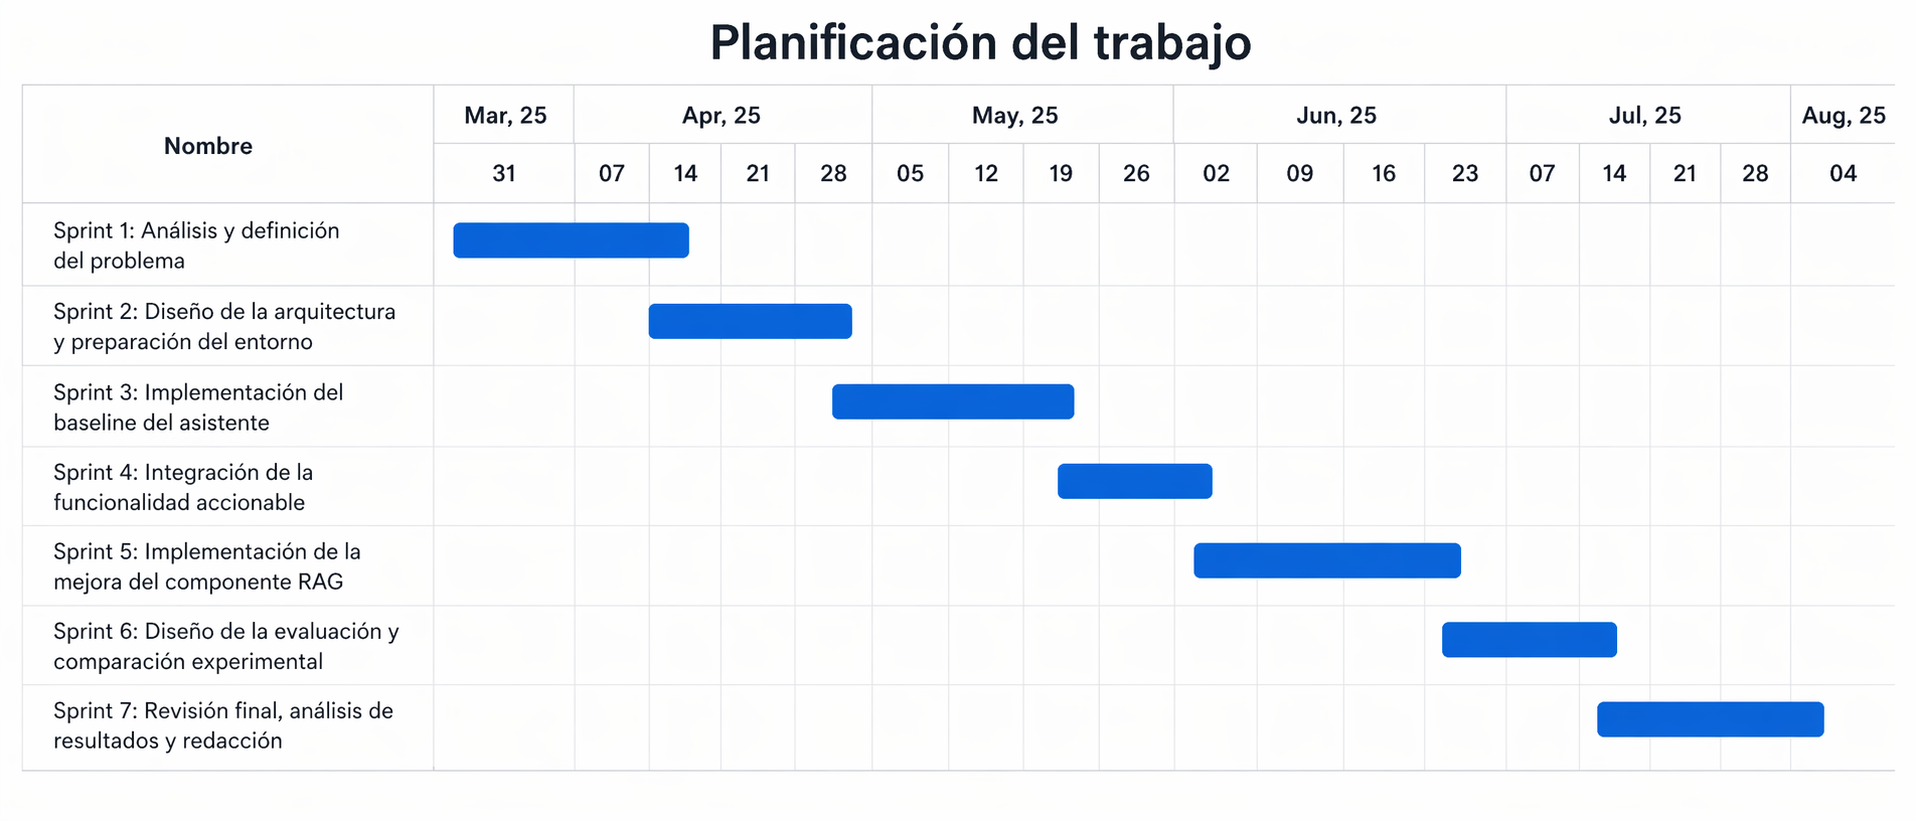
\includegraphics[width=1\textwidth]{contenido/imagenes/Gantt.png}
    \caption{Diagrama de Gantt con la planificación temporal del trabajo.}
    \label{fig:gantt}
\end{figure}

\section{Recursos y costes}\label{sec:recursos}

En esta sección se describen los recursos necesarios y se realiza una estimación orientativa de sus costes. 
Dado que se trata de un proyecto académico desarrollado de forma individual, la mayor parte del esfuerzo recae en la estudiante, mientras que la dirección del TFM asume funciones de supervisión, revisión y seguimiento. 

\subsection{Recursos humanos}

Los recursos humanos considerados para el desarrollo del proyecto son los siguientes:

\begin{itemize}
    \item \textbf{Dirección del TFM}: responsable de orientar el trabajo, revisar su evolución, validar las decisiones principales y supervisar la coherencia metodológica y académica del proyecto.
    
    \item \textbf{Estudiante}: responsable del análisis del problema, diseño de la arquitectura, implementación del prototipo, preparación del conjunto de evaluación, ejecución de los experimentos, análisis de resultados y redacción de la memoria final.
\end{itemize}

Aunque el proyecto es realizado por una única persona, desde el punto de vista de la estimación puede considerarse que la estudiante asume varias funciones de forma simultánea, entre ellas las de analista, desarrolladora e investigadora aplicada.

\subsection{Recursos técnicos}

Para el desarrollo del TFM se requerirán los siguientes recursos técnicos:

\begin{itemize}
    \item Ordenador personal para desarrollo, pruebas y redacción de la memoria.
    \item Entorno de programación y herramientas de desarrollo para la implementación del prototipo.
    \item Herramientas de edición y documentación para la elaboración de diagramas, esquemas y memoria.
    \item Servicios o librerías necesarios para la implementación del sistema RAG, la integración del modelo generativo y el procesamiento documental.
    \item Herramientas de evaluación y análisis de resultados.
\end{itemize}

En términos generales, se priorizará el uso de herramientas gratuitas, académicas o ya disponibles en el entorno de trabajo, por lo que no se prevé un coste material elevado asociado al proyecto. 
En caso de utilizar servicios externos de pago, estos quedarán limitados a un uso puntual o experimental.

\subsection{Estimación de dedicación}

La siguiente tabla recoge una estimación orientativa de las horas de trabajo necesarias para desarrollar el proyecto:

\begin{table}[H]
\centering
\begin{tabular}{lccc}
\toprule
\textbf{Rol} & \textbf{Horas proyecto} & \textbf{Horas memoria} & \textbf{Total horas} \\
\midrule
Estudiante & 300 & 120 & 420 \\
Dirección del TFM & 20 & 10 & 30 \\
\bottomrule
\end{tabular}
\caption{Estimación de horas dedicadas al proyecto.}
\label{tab:horas_proyecto}
\end{table}

La dedicación principal corresponde a la estudiante, ya que asume tanto el desarrollo técnico del prototipo como la parte experimental y documental del trabajo. 
En cambio, la dirección del TFM participa de manera periódica mediante reuniones de seguimiento, revisión de avances y supervisión de la memoria.

\subsection{Estimación de costes}

A efectos de estimación, se asigna un coste por hora orientativo a cada uno de los roles considerados. Estos valores no deben interpretarse como costes contractuales reales, sino como una aproximación académica al esfuerzo invertido en el proyecto.

\begin{table}[H]
\centering
\begin{tabular}{lccc}
\toprule
\textbf{Rol} & \textbf{Total horas} & \textbf{Coste/hora (€)} & \textbf{Coste total (€)} \\
\midrule
Estudiante & 420 & 25 & 10.500 \\
Dirección del TFM & 30 & 35 & 1.050 \\
\midrule
\textbf{Total} & \textbf{450} & -- & \textbf{11.550} \\
\bottomrule
\end{tabular}
\caption{Estimación orientativa de costes humanos del proyecto.}
\label{tab:costes_proyecto}
\end{table}

Por tanto, el coste total estimado del proyecto, considerando únicamente los recursos humanos, sería de 11.550\,€. 
Esta cifra representa una valoración aproximada del esfuerzo necesario para desarrollar el asistente, implementar la mejora experimental propuesta y documentar adecuadamente el trabajo realizado.


        \chapter{Diseño e implementación de la propuesta}\label{chap:diseno-implementacion}

En este capítulo se describe el diseño técnico del asistente institucional propuesto, así como las principales decisiones adoptadas durante su implementación. 
Para ello, se presenta la arquitectura general del sistema, el flujo de ejecución del asistente, el papel del agente orquestador y las herramientas disponibles. 
Finalmente, se exponen las variantes implementadas y las tecnologías utilizadas para el desarrollo del prototipo.

\section{Arquitectura general del sistema}\label{sec:arquitectura-general}

La arquitectura general del sistema se organiza en torno a dos fases principales: una fase offline de preparación del corpus y una fase online de ejecución del asistente. 
Esta separación permite distinguir claramente entre las tareas necesarias para construir la base documental y las tareas que se realizan en tiempo de consulta.

La fase offline comprende la obtención, normalización, segmentación e indexación de los documentos que forman parte del corpus institucional. 
En esta etapa, las fuentes documentales se recopilan a partir de páginas y documentos públicos, se transforman a un formato homogéneo, se dividen en fragmentos o \textit{chunks} y se enriquecen con metadatos. 
Posteriormente, dichos fragmentos se representan mediante embeddings y se almacenan en una base documental preparada para su recuperación posterior.

La fase online comienza cuando el usuario introduce una consulta en la interfaz conversacional. 
A partir de esa entrada, el agente orquestador interpreta la petición y decide qué capacidades del sistema deben activarse. 
En consultas informativas, el flujo principal consiste en recuperar evidencia documental relevante y generar una respuesta fundamentada. 
En cambio, cuando la petición tiene una intención accionable, el orquestador puede activar una herramienta específica, como la generación de un borrador de correo.

La Figura~\ref{fig:arquitectura-general} muestra una visión global de esta arquitectura. 
En ella se observa cómo la base documental alimenta la herramienta de recuperación, cómo el orquestador coordina las capacidades disponibles y cómo la capa de observabilidad permite registrar trazas del comportamiento del sistema durante la ejecución.

\section{Flujo de ejecución del asistente}\label{sec:flujo-ejecucion}

El flujo de ejecución del asistente parte de una consulta formulada en lenguaje natural por el usuario. 
La entrada se recibe a través de la interfaz conversacional y se envía al núcleo del sistema, donde el orquestador determina el tipo de tarea que debe resolverse. 
Esta decisión condiciona el resto del proceso, ya que no todas las consultas requieren el mismo tratamiento.

En el caso de preguntas informativas simples, el sistema sigue un flujo RAG directo. 
Primero, la consulta se transforma en una representación adecuada para el recuperador. 
Después, se buscan los fragmentos documentales más relevantes dentro de la base documental. 
Finalmente, el modelo de lenguaje genera una respuesta utilizando como contexto la evidencia recuperada.

Cuando la consulta requiere combinar información de varias fuentes, el sistema puede descomponer la pregunta en subconsultas o recuperar un conjunto más amplio de fragmentos candidatos. 
Este comportamiento resulta útil en preguntas comparativas o en consultas que no pueden resolverse a partir de un único documento. 
En estos casos, el objetivo no es únicamente recuperar un fragmento aislado, sino reunir evidencia suficiente para elaborar una respuesta más completa y estructurada.

En las preguntas no respondibles, el sistema debe evitar generar una respuesta no fundamentada. 
Por ello, si la evidencia recuperada no resulta suficiente o no guarda relación clara con la consulta, el flujo debe favorecer la abstención o una respuesta prudente que indique la falta de información disponible en el corpus. 
Este comportamiento es especialmente importante en un asistente institucional, donde proporcionar información incorrecta podría afectar negativamente a la confianza del usuario.

Por último, cuando la consulta expresa una intención accionable, como solicitar ayuda para redactar un correo formal, el orquestador activa la herramienta correspondiente. 
En esta versión del prototipo, dicha acción se limita a la generación de un borrador, manteniendo siempre una separación explícita entre proponer una acción y ejecutarla realmente.

\section{Papel del orquestador}\label{sec:papel-orquestador}

El agente orquestador actúa como componente de coordinación dentro del sistema. 
Su función principal consiste en interpretar la consulta del usuario, decidir qué flujo de ejecución resulta más adecuado y activar las herramientas necesarias para resolver la tarea. 
De este modo, el orquestador no sustituye al componente de recuperación ni al modelo de lenguaje, sino que organiza su uso dentro de una arquitectura controlada.

Desde una perspectiva agéntica, cada consulta se trata como una tarea que puede requerir distintos pasos. 
Algunas preguntas pueden resolverse mediante una recuperación documental directa, mientras que otras requieren comparar información, dividir la consulta en partes o activar una herramienta accionable. 
El orquestador permite introducir esta lógica de decisión sin acoplarla directamente al recuperador ni al modelo generativo.

En el prototipo, el orquestador contempla principalmente cinco tipos de comportamiento. 
En primer lugar, puede delegar una consulta simple al flujo RAG determinista. 
En segundo lugar, puede tratar consultas multi-documento mediante una estrategia más estructurada. 
En tercer lugar, puede organizar respuestas comparativas diferenciando entidades, criterios o condiciones. 
En cuarto lugar, puede abstenerse ante consultas no respondibles cuando no existe evidencia suficiente en el corpus. 
Finalmente, puede activar la herramienta de generación de borradores cuando detecta una petición orientada a acción.

Esta separación aporta trazabilidad y control al sistema. 
En lugar de generar siempre una respuesta del mismo modo, el asistente puede adaptar el flujo a la naturaleza de la consulta. 
Además, permite evaluar de forma independiente el impacto del orquestador sobre dimensiones como la abstención, la selección de herramientas y la estructuración de respuestas.

Para reforzar este control, el orquestador define un conjunto explícito de acciones permitidas que delimitan el ámbito de actuación del asistente.
En concreto, las acciones válidas son las siguientes: respuesta informativa sobre un único documento (\texttt{answer\_with\_rag}), respuesta informativa que combina evidencia de múltiples fuentes (\texttt{multi\_step\_rag}), respuesta comparativa entre entidades o documentos (\texttt{comparative\_rag}), generación supervisada de un borrador de correo electrónico (\texttt{draft\_email}) y abstención explícita cuando la consulta no puede responderse con la evidencia disponible en el corpus (\texttt{refuse}).
Cualquier consulta cuya intención quede fuera de este conjunto predefinido es rechazada antes de activar herramientas o iniciar la generación, convirtiendo al orquestador en una primera capa de \textit{guardrails} del sistema.
Este mecanismo evita que el asistente procese peticiones fuera del dominio definido, como solicitudes ajenas al ámbito institucional, peticiones que impliquen acciones no supervisadas o consultas que no puedan fundamentarse en el corpus documental disponible.

\section{Herramientas disponibles}\label{sec:herramientas-disponibles}

El sistema incorpora herramientas especializadas que pueden ser utilizadas por el orquestador durante la ejecución. 
En el contexto de este trabajo, una herramienta se entiende como un componente externo al modelo de lenguaje que proporciona una capacidad concreta, como recuperar información documental o generar una salida accionable.

La herramienta principal es la recuperación documental. 
Esta herramienta permite consultar la base documental construida previamente y devolver los fragmentos más relevantes para la pregunta del usuario. 
Su papel es fundamental en el sistema, ya que proporciona la evidencia necesaria para que las respuestas estén fundamentadas en información del corpus y no dependan únicamente del conocimiento paramétrico del modelo de lenguaje.

La segunda herramienta es la generación de borradores de correo. 
Esta funcionalidad permite transformar una consulta del usuario o una respuesta informativa previa en un texto formal orientado a una actuación posterior. 
En esta versión del prototipo, la herramienta se mantiene en modo simulado o \textit{mockeado}: el sistema genera el borrador, pero no envía ningún mensaje real. 
Esta decisión permite validar el flujo conversacional y la utilidad de la salida generada sin introducir riesgos asociados al envío automático de correos.

El uso de herramientas se plantea de forma supervisada. 
El asistente puede proponer una acción, preparar un borrador o estructurar una respuesta accionable, pero la ejecución efectiva queda bajo control del usuario. 
Este enfoque resulta adecuado para un entorno institucional, donde es importante mantener trazabilidad, evitar acciones no deseadas y conservar la intervención humana en decisiones sensibles.

\section{Variantes implementadas}\label{sec:variantes-implementadas}

Con el fin de evaluar el impacto de los distintos componentes del sistema, se implementaron varias variantes del prototipo. 
Estas variantes permiten comparar una configuración inicial sencilla con versiones que incorporan mejoras específicas en la recuperación documental o en el control del flujo mediante orquestación.

La primera variante corresponde al \textit{baseline} determinista. 
Esta configuración sigue un flujo RAG directo: recibe la consulta del usuario, recupera fragmentos mediante búsqueda semántica y genera una respuesta a partir del contexto obtenido. 
Su objetivo es servir como punto de referencia para analizar el efecto de las mejoras posteriores.

La segunda variante introduce una mejora en el componente de recuperación de información. 
En este caso, la búsqueda semántica se complementa con recuperación léxica mediante BM25 y con una etapa posterior de \textit{reranking}. 
El objetivo de esta variante es comprobar si una recuperación más robusta permite situar la evidencia relevante en posiciones más altas del ranking y, por tanto, mejorar la calidad del contexto proporcionado al modelo de lenguaje.

La tercera variante incorpora el agente orquestador. 
En esta configuración, el sistema no aplica siempre el mismo flujo de forma determinista, sino que clasifica la consulta y decide cómo resolverla. 
Esta variante permite analizar el valor del orquestador en tareas como la abstención ante preguntas no respondibles, la identificación de solicitudes accionables y la activación de herramientas.

Una mejora relevante incorporada en la lógica del orquestador es la capacidad de gestionar consultas ambiguas o poco concretas. Cuando el sistema detecta que la pregunta del usuario carece de suficiente especificidad, no se limita a solicitar una aclaración, sino que primero genera una respuesta general basada en la evidencia disponible y, a continuación, plantea una pregunta de clarificación. De este modo, el usuario recibe información útil de inmediato y se fomenta un diálogo iterativo que permite afinar la respuesta en pasos sucesivos. Esta funcionalidad mejora la experiencia conversacional, ya que combina la entrega de valor inmediato con la capacidad de guiar al usuario hacia consultas más precisas, optimizando así la utilidad del asistente en escenarios reales donde las preguntas iniciales suelen ser vagas o incompletas.

Estas variantes se implementan de forma configurable, permitiendo activar o desactivar componentes como la recuperación híbrida, el \textit{reranking} o el orquestador. 
Esta decisión facilita la comparación experimental posterior, ya que cada configuración puede ejecutarse sobre el mismo corpus y el mismo conjunto de consultas de evaluación.

Una vez descrito el diseño general del sistema, las siguientes secciones presentan las principales tecnologías utilizadas para implementar el prototipo. 
La selección se ha realizado atendiendo a criterios de modularidad, facilidad de integración, bajo coste, posibilidad de ejecución local y adecuación al desarrollo de sistemas basados en recuperación de información y modelos de lenguaje.

\section{Lenguaje y entorno de desarrollo y ejecución}\label{sec:entorno-desarrollo}

\subsection{Python}\label{subsec:python}

El lenguaje principal del proyecto es Python. 
Esta elección se debe a su amplia adopción en el ámbito de la inteligencia artificial, el procesamiento del lenguaje natural y la computación científica. 
Su ecosistema incluye bibliotecas consolidadas para el tratamiento de datos, el aprendizaje automático y el uso de modelos de lenguaje, como NumPy, SciPy, scikit-learn o Transformers \cite{harris2020array, virtanen2020scipy, pedregosa2011scikit, wolf2020transformers}. 
Esta disponibilidad de herramientas resulta especialmente adecuada para un prototipo basado en RAG, donde es necesario integrar procesamiento documental, generación de embeddings, recuperación semántica, reranking, evaluación y conexión con modelos generativos.
Además, el uso de entornos virtuales y variables de configuración permite aislar dependencias y modificar parámetros del sistema sin alterar el código fuente, lo que facilita la reproducibilidad de las pruebas.

Frente a lenguajes como Java o Go, Python ofrece una curva de desarrollo más rápida y una integración más directa con las principales librerías utilizadas en proyectos de NLP y aprendizaje automático. 
Java y Go son alternativas robustas para servicios backend con altos requisitos de concurrencia, mantenibilidad o rendimiento. 
Sin embargo, en este trabajo el objetivo principal no es optimizar una infraestructura de producción, sino diseñar, implementar y evaluar distintas variantes de una arquitectura RAG. 

También se ha valorado el uso de lenguajes de menor nivel, como C++, que podrían aportar ventajas en términos de rendimiento. 
No obstante, gran parte del coste computacional del sistema recae en la inferencia de modelos, la generación de embeddings y las consultas al almacén vectorial, componentes que ya suelen estar implementados mediante bibliotecas optimizadas o servicios externos.
 Por tanto, utilizar C++ para la lógica de orquestación o experimentación aumentaría la complejidad del desarrollo sin aportar una mejora proporcional al objetivo del prototipo.

Otro aspecto relevante es la reproducibilidad. 
Python permite aislar dependencias mediante entornos virtuales, de forma que cada entorno puede mantener sus propios paquetes y versiones sin interferir con la instalación global del sistema \cite{pep405}. 
Esta característica facilita la ejecución controlada del prototipo, la comparación entre variantes experimentales y la futura replicación del trabajo.

\subsection{Docker}\label{subsec:docker}

Docker se utiliza como tecnología de contenedorización para ejecutar de forma aislada los servicios auxiliares del sistema. 
En el contexto de este proyecto, su uso permite levantar componentes como Qdrant, utilizado como base de datos vectorial, y Phoenix, empleado para la observabilidad del pipeline, sin instalarlos directamente sobre el sistema operativo anfitrión.

Para la definición y ejecución de estos servicios se emplea Docker Compose, que permite describir en un único fichero de configuración los servicios, redes y volúmenes necesarios para una aplicación multicontenedor \cite{dockerCompose}. 
El uso de volúmenes permite conservar información entre ejecuciones, evitando que datos como las colecciones vectoriales o las trazas generadas se pierdan al detener o recrear los contenedores \cite{dockerVolumes}. 
Esta característica resulta especialmente útil en un prototipo RAG, donde es necesario mantener el estado de servicios persistentes durante las fases de ingesta, evaluación y experimentación.

En comparación con una instalación manual de cada servicio, Docker reduce la dependencia de configuraciones específicas del equipo de desarrollo y simplifica la preparación del entorno. 

\section{Procesamiento documental}\label{sec:procesamiento-documental}

El procesamiento documental constituye una fase esencial del sistema, ya que condiciona la calidad de la información que posteriormente será recuperada por el modelo. 
En este proyecto, dicha fase incluye la obtención de documentos, su conversión a un formato homogéneo y su segmentación en fragmentos adecuados para la recuperación semántica.

\subsection{Obtención del corpus y scraping web}\label{subsec:obtencion-corpus}

El corpus del proyecto se construye exclusivamente a partir de información disponible en URLs públicas del dominio institucional. Para ello, se desarrolló un proceso de scraping propio basado en \textit{httpx} y \textit{BeautifulSoup}. La primera librería se utilizó para realizar peticiones HTTP de forma controlada, mientras que la segunda permitió analizar el contenido HTML, extraer el texto principal de las páginas y eliminar elementos no relevantes para la recuperación, como menús de navegación, pies de página, scripts o bloques puramente visuales.

El proceso de obtención del corpus no se planteó como un crawler generalista, sino como una recopilación acotada y reproducible de fuentes alineadas con el caso de uso del asistente institucional. Para ello, se partió de un conjunto inicial de URLs semilla seleccionadas manualmente por su relevancia para consultas habituales del dominio universitario, incluyendo información sobre trámites académicos, prácticas, becas, normativas, procedimientos administrativos y servicios para estudiantes.

Durante la recopilación se aplicaron criterios de inclusión y exclusión. Se incluyeron aquellas páginas que contenían información institucional textual, estable, verificable y potencialmente útil para responder preguntas del usuario. En cambio, se descartaron páginas que no superaban un umbral mínimo de 80 palabras de contenido útil tras la limpieza del HTML, páginas cuyo contenido quedaba compuesto mayoritariamente por elementos de navegación, banners o bloques visuales sin valor informativo, y páginas con contenido promocional o de actualidad desconectado del dominio de consulta. Esta selección permitió construir un corpus más reducido, pero más controlado y coherente con los objetivos experimentales del trabajo.

El proceso de limpieza del HTML incluyó la eliminación sistemática de etiquetas de navegación (\texttt{nav}), cabeceras (\texttt{header}), pies de página (\texttt{footer}), formularios, barras laterales y bloques de JavaScript o CSS. Adicionalmente, se filtraron bloques HTML con atributos de clase o identificador asociados a patrones habituales de ruido en sitios web institucionales, como menús, \textit{banners}, gestión de \textit{cookies}, noticias, eventos, contenido social o elementos promocionales. Tras este proceso, únicamente se conservó el contenido principal de cada página, extraído preferentemente del elemento \texttt{main} o \texttt{article} cuando estuvo disponible. El cumplimiento del fichero \texttt{robots.txt} se verificó antes de cada descarga y se respetó un retardo mínimo entre peticiones para no sobrecargar los servidores.

Como resultado, de las 30 páginas descargadas correctamente, 4 fueron descartadas: tres no alcanzaron el umbral mínimo de palabras tras la limpieza y una presentó contenido mayoritariamente visual o estructural sin texto útil recuperable. Los 26 documentos restantes constituyen el corpus final empleado en la evaluación.

Además, el proceso se diseñó teniendo en cuenta criterios de reproducibilidad y trazabilidad. Cada documento recuperado conserva metadatos asociados a su fuente original, como la URL, el título, la categoría temática y el identificador del documento. Estos metadatos permiten posteriormente relacionar cada fragmento recuperado con su origen, analizar errores de recuperación y mostrar las fuentes utilizadas en las respuestas generadas por el asistente.

Como resultado de este proceso, el corpus final quedó formado por documentos institucionales públicos transformados a un formato textual homogéneo y preparados para su segmentación e indexación. Esta fase resulta especialmente relevante dentro del proyecto, ya que la calidad del corpus condiciona directamente la calidad de la recuperación documental y, por tanto, la fundamentación de las respuestas generadas por el sistema.

\begin{table}[H]
\centering
\begin{tabular}{lr}
\hline
\textbf{Elemento} & \textbf{Valor} \\
\hline
URLs semilla consideradas & 30 \\
Páginas descargadas correctamente & 30 \\
Páginas descartadas durante la limpieza & 4 \\
Documentos finales incorporados al corpus & 26 \\
Formato final de almacenamiento & Markdown \\
Tamaño medio de documento & 1557,92 palabras \\
Chunks generados & 520 \\
Tamaño medio de chunk & 851 caracteres \\
\hline
\end{tabular}
\caption{Resumen del proceso de construcción del corpus documental.}
\label{tab:resumen_corpus}
\end{table}

\subsection{Conversión y normalización de documentos}\label{subsec:conversion-normalizacion}

Una vez obtenidos los documentos, se aplica un proceso de normalización para reducir la heterogeneidad entre formatos. 
Las páginas HTML se convierten a Markdown mediante \texttt{markdownify}, lo que permite conservar una estructura textual sencilla y legible, eliminando al mismo tiempo elementos propios de la presentación web que no aportan información relevante para la recuperación \cite{markdownify}.

En el caso de documentos PDF, se utiliza PyMuPDF, una librería orientada a la extracción, análisis y manipulación de documentos PDF desde Python \cite{pymupdf}.
A diferencia de las fuentes HTML, los documentos PDF no se convierten a formato Markdown: su contenido textual se extrae directamente como texto plano, sin ninguna conversión de formato intermedia.
Los ficheros de texto plano y Markdown se procesan directamente en su formato original.
En definitiva, el formato Markdown se aplica exclusivamente a los documentos procedentes del \textit{scraping} web, donde el proceso genera ficheros \texttt{.md} enriquecidos con metadatos en cabecera; para las fuentes PDF o de texto plano, el contenido se trata directamente sin conversión adicional.
Este flujo permite transformar distintas fuentes en texto recuperable, facilitando las etapas posteriores de segmentación e indexación.

\subsection{Segmentación del corpus y metadatos}\label{subsec:chunking-metadatos}

Tras la normalización, los documentos se dividen en fragmentos o \textit{chunks}. 
Esta segmentación es necesaria porque los modelos de embeddings y los modelos generativos trabajan con límites de contexto, y porque la recuperación resulta más precisa cuando se indexan unidades de información de tamaño controlado en lugar de documentos completos.

En este proyecto, la segmentación sigue una estrategia jerárquica orientada a preservar la coherencia semántica de los textos.
En primer lugar, el documento se divide por límites de párrafo, identificados como bloques separados por una o más líneas en blanco.
Si un párrafo supera el tamaño máximo de fragmento establecido (900 caracteres), se aplica una segunda división por oraciones mediante el reconocimiento de signos de puntuación terminal.
En caso de que una oración individual resulte todavía demasiado larga, se recurre a una división por palabras como último recurso.
Los fragmentos resultantes se construyen acumulando unidades hasta alcanzar el tamaño objetivo de 800 caracteres, con un margen entre 600 y 900 caracteres.
Para evitar la pérdida de contexto entre fragmentos consecutivos, se aplica un solapamiento de 150 caracteres, de modo que el final de un fragmento se reutiliza como inicio del siguiente.

Esta estrategia jerárquica se prefiere frente a alternativas más simples por varias razones.
La división por tamaño fijo de caracteres o \textit{tokens}, pese a ser la opción más directa, produce cortes arbitrarios que pueden interrumpir una oración, una enumeración o un concepto compuesto, lo que perjudica tanto la representación semántica del \textit{embedding} como la coherencia del contexto proporcionado al modelo generativo.
La división únicamente por oraciones genera fragmentos excesivamente pequeños que pueden carecer de contexto suficiente para que el recuperador comprenda el significado completo del pasaje.
La segmentación únicamente por párrafos, sin control del tamaño máximo, puede producir fragmentos demasiado largos que superen la ventana de contexto útil del modelo de \textit{embeddings} y diluyan la señal semántica en la representación vectorial.
La estrategia adoptada busca un equilibrio entre estas restricciones, preservando la coherencia textual siempre que sea posible dentro de los límites de tamaño impuestos.

Además, cada fragmento conserva metadatos asociados a su documento de origen, lo que permite mantener la trazabilidad de las respuestas y recuperar la fuente original de la información utilizada por el sistema.

\section{Almacenamiento vectorial}\label{sec:almacenamiento-vectorial}

En los sistemas RAG, el almacenamiento vectorial permite guardar las representaciones numéricas de los fragmentos documentales y recuperarlos posteriormente mediante búsqueda por similitud semántica. 
Para esta función se ha seleccionado Qdrant, una base de datos vectorial orientada a la búsqueda semántica y al almacenamiento de vectores junto con información adicional o \textit{payload} \cite{qdrantDocs}.

La elección de Qdrant se justifica por varias razones. 
En primer lugar, permite ejecutarse de forma local mediante Docker, lo que encaja con el enfoque de bajo coste y control del entorno planteado para el prototipo. 
En segundo lugar, ofrece persistencia de datos, filtrado por metadatos y una API de consulta que facilita su integración con el pipeline RAG. 
Estas características resultan especialmente útiles cuando se desea recuperar fragmentos no solo por similitud vectorial, sino también teniendo en cuenta información asociada a la fuente, el documento o la categoría del contenido.

Se valoraron otras alternativas ampliamente utilizadas en el ámbito de la recuperación vectorial. 
FAISS constituye una opción eficiente para búsqueda de similitud y clustering sobre vectores densos, pero se plantea principalmente como una librería y no como una base de datos vectorial completa con servicio persistente y API propia \cite{faissDocs}. 
Chroma, por su parte, ofrece una solución sencilla para almacenar embeddings, realizar búsquedas vectoriales y filtrar por metadatos \cite{chromaDocs}. 
Sin embargo, Qdrant se ajusta mejor a las necesidades del proyecto al proporcionar una separación más clara entre el servicio de almacenamiento vectorial y el resto de componentes del sistema.

También se consideraron soluciones como Pinecone y Weaviate. 
Pinecone ofrece una base de datos vectorial gestionada orientada a aplicaciones de IA en producción \cite{pineconeDocs}, mientras que Weaviate proporciona una base de datos vectorial de código abierto con capacidades de búsqueda semántica e híbrida \cite{weaviateDocs}. 
No obstante, para este trabajo se prioriza una solución que pueda ejecutarse localmente, sin costes asociados por uso y con suficiente flexibilidad para las fases de ingesta, recuperación y evaluación. 

La Tabla~\ref{tab:comparativa_vectoriales} resume las principales características de las alternativas consideradas.

\begin{table}[H]
\centering
\begin{tabular}{lcccc}
\hline
\textbf{Sistema} & \textbf{Tipo} & \textbf{Persistencia} & \textbf{API propia} & \textbf{Ejecución local} \\
\hline
Qdrant & BD vectorial & Sí & Sí & Sí (Docker) \\
FAISS & Librería de indexación & Manual & No & Sí \\
Chroma & BD vectorial ligera & Sí & Sí & Sí \\
Pinecone & BD vectorial gestionada & Sí (cloud) & Sí & No \\
Weaviate & BD vectorial OSS & Sí & Sí & Sí \\
\hline
\end{tabular}
\caption{Comparativa de bases de datos vectoriales consideradas para el proyecto.}
\label{tab:comparativa_vectoriales}
\end{table}

\section{Modelos de representación semántica}\label{sec:rep-semantica}

Los modelos de representación semántica permiten transformar consultas y fragmentos documentales en vectores numéricos, de forma que puedan compararse mediante medidas de similitud. 
Esta representación es uno de los componentes principales de una arquitectura RAG, ya que determina en gran medida qué información será recuperada y utilizada posteriormente por el modelo generativo.

\subsection{BGE-M3}\label{subsec:embeddings}

Para la generación de embeddings se ha seleccionado BGE-M3, publicado por el Beijing Academy of Artificial Intelligence (BAAI) e integrado mediante la librería \texttt{SentenceTransformers} \cite{chen2024bgem3}.
Este modelo ha sido diseñado para tareas de recuperación multilingüe y destaca por su triple enfoque: \textit{multi-lingual} (soporte para más de cien idiomas), \textit{multi-functionality} (capacidad para producir representaciones densas, dispersas y multi-vector) y \textit{multi-granularity} (ventana de contexto de hasta 8192 tokens).

Desde el punto de vista arquitectónico, BGE-M3 utiliza XLM-RoBERTa-Large como columna vertebral, lo que resulta en aproximadamente 570 millones de parámetros.
Su salida por defecto es un vector denso de 1024 dimensiones que captura el significado semántico del texto de entrada y puede compararse mediante similitud coseno con los vectores de los fragmentos del corpus.
Esta arquitectura permite, además, combinar la representación densa con señales de recuperación dispersa o multi-vector cuando el pipeline lo requiere.

Se evaluaron otras alternativas antes de seleccionar BGE-M3.
\textit{multilingual-e5-large}, de Microsoft, ofrece un tamaño inferior (560 millones de parámetros, vectores de 1024 dimensiones) con un buen rendimiento multilingüe, pero su cobertura en español es más limitada que la de BGE-M3 en benchmarks de recuperación \cite{wang2024multilingual}.
Modelos como \textit{paraphrase-multilingual-mpnet-base-v2} son más ligeros (278 millones de parámetros, 768 dimensiones), pero su capacidad de representación semántica es inferior para tareas de recuperación precisas.
Las APIs de embeddings de OpenAI (\textit{text-embedding-3-small} y \textit{text-embedding-3-large}) ofrecen alta calidad, pero introducen dependencia de servicios externos y coste por uso, lo que resulta incompatible con el enfoque de ejecución local y bajo coste del prototipo.
En conjunto, BGE-M3 ofrece el mejor equilibrio entre calidad de recuperación, soporte del español, tamaño manejable y posibilidad de ejecución local para los objetivos del proyecto.

\section{Recuperación de información}\label{sec:recuperacion-informacion}

La recuperación de información es el proceso mediante el cual el sistema selecciona los fragmentos documentales más relevantes para una consulta. 
En el prototipo se contempla una recuperación densa basada en embeddings y una variante híbrida que combina similitud semántica con recuperación léxica.

\subsection{Recuperación semántica}\label{subsec:recuperacion-semantica}

La recuperación semántica se realiza generando el embedding de la consulta y comparándolo con los vectores previamente almacenados en la base de datos vectorial. 
De esta forma, el sistema puede recuperar fragmentos relacionados por significado, aunque no compartan exactamente los mismos términos que la pregunta del usuario.

Este enfoque resulta especialmente útil en un asistente conversacional, ya que las consultas suelen formularse de manera natural y pueden diferir de la redacción exacta presente en los documentos del corpus.

Cabe señalar que en los agentes conversacionales es habitual incorporar una etapa previa de \textit{query rewriting}, consistente en reformular la consulta del usuario antes de lanzarla contra el índice documental \cite{ma2023queryrewriting}.
Esta técnica permite adaptar el lenguaje natural de la pregunta al vocabulario del corpus, desambiguar referencias contextuales en conversaciones de múltiples turnos y mejorar la cobertura de recuperación.
En el prototipo presentado no se ha implementado esta etapa, ya que el sistema opera en modo de un único turno por consulta, eliminando la necesidad de resolver referencias a contexto previo.
Sin embargo, su incorporación constituiría una mejora natural del sistema en un escenario conversacional multi-turno.

\subsection{Recuperación híbrida con BM25}\label{subsec:recuperacion-hibrida}

Además de la recuperación densa, el sistema contempla una variante híbrida que combina la similitud vectorial con BM25 (\textit{Best Match 25}), un modelo probabilístico clásico de recuperación léxica basado en coincidencia de términos y ponderación estadística \cite{robertson2009bm25}.

BM25 asigna a cada documento $D$ una puntuación respecto a una consulta $Q$ con términos $q_1, \ldots, q_n$ según la expresión:

\begin{equation}
\text{score}(D, Q) = \sum_{i=1}^{n} \text{IDF}(q_i) \cdot \frac{f(q_i, D) \cdot (k_1 + 1)}{f(q_i, D) + k_1 \cdot \left(1 - b + b \cdot \frac{|D|}{\text{avgdl}}\right)}
\label{eq:bm25}
\end{equation}

donde $f(q_i, D)$ es la frecuencia del término $q_i$ en el documento $D$, $|D|$ es la longitud del documento en número de términos, $\text{avgdl}$ es la longitud media de los documentos de la colección, $k_1$ y $b$ son hiperparámetros de ajuste (valores típicos: $k_1 = 1{,}5$, $b = 0{,}75$), e $\text{IDF}(q_i) = \log\frac{N - n(q_i) + 0{,}5}{n(q_i) + 0{,}5}$ penaliza los términos que aparecen en muchos documentos, siendo $N$ el número total de documentos y $n(q_i)$ el número de documentos que contienen el término $q_i$.

Este mecanismo tiene dos propiedades relevantes para el sistema. El factor IDF premia los términos infrecuentes en la colección, como nombres de trámites, titulaciones o conceptos administrativos específicos, que suelen ser señales discriminativas en consultas institucionales. El factor de normalización por longitud evita que los documentos más largos sean sistemáticamente favorecidos frente a documentos más cortos pero igualmente relevantes.

En la variante híbrida, las puntuaciones de BM25 y de similitud vectorial se normalizan de forma independiente y se combinan mediante una suma ponderada con pesos ajustables. Esta combinación permite equilibrar las ventajas de la búsqueda semántica —que captura relaciones por significado incluso sin coincidencia léxica— con la precisión de BM25 ante términos específicos, mejorando la robustez del sistema ante distintos tipos de preguntas.

\section{Mejora de la recuperación mediante reranking}\label{sec:reranking}

El reranking se introduce como una segunda etapa de recuperación.
Tras obtener un conjunto inicial de fragmentos candidatos mediante recuperación semántica o híbrida, un modelo adicional vuelve a ordenar dichos fragmentos en función de su relevancia respecto a la consulta.
Esta etapa permite corregir el orden inicial cuando los métodos de primera etapa no han situado los fragmentos más relevantes en las posiciones superiores del ranking.

Los modelos de reranking pueden clasificarse en tres categorías según su estrategia de puntuación \cite{liu2009learning}.
Los modelos \textit{pointwise} asignan una puntuación independiente a cada par formado por la consulta y un fragmento candidato, tratando el problema como una tarea de clasificación o regresión sobre ejemplos individuales.
Los modelos \textit{pairwise} comparan fragmentos de dos en dos, aprendiendo a determinar cuál es más relevante en cada comparación.
Los modelos \textit{listwise} optimizan directamente la ordenación de toda la lista de candidatos de forma conjunta.

En este proyecto se opta por un enfoque \textit{pointwise} (configuración \textit{cross-encoder}) por varias razones.
En primer lugar, este enfoque asigna una puntuación de relevancia absoluta a cada fragmento de forma independiente, lo que simplifica la integración en el pipeline y permite ajustar umbrales de corte de forma controlada.
En segundo lugar, su complejidad escala linealmente con el número de fragmentos candidatos, lo que lo hace más eficiente que los enfoques \textit{listwise} para un tamaño de lista moderado.
Por último, existen modelos preentrenados de alta calidad para esta configuración que pueden ejecutarse localmente sin entrenamiento adicional.

\subsection{Modelo de reranking seleccionado}\label{subsec:modelo-reranking}

Para esta tarea se emplea un modelo de tipo \texttt{CrossEncoder} integrado mediante \texttt{SentenceTransformers}.
A diferencia de los modelos bi-encoder utilizados para generar embeddings de forma independiente, un \texttt{CrossEncoder} evalúa conjuntamente el par formado por la consulta y cada fragmento candidato, lo que permite obtener una estimación más precisa de su relevancia \cite{sentenceTransformersCrossEncoder}.

El modelo seleccionado es \textit{BAAI/bge-reranker-v2-m3}, publicado por el Beijing Academy of Artificial Intelligence (BAAI) y diseñado específicamente para tareas de reranking multilingüe \cite{chen2024bgem3}.
Se trata de un modelo transformer de tipo encoder, entrenado mediante aprendizaje contrastivo sobre pares de consultas y pasajes relevantes e irrelevantes en múltiples idiomas.
A diferencia del modelo de embeddings BGE-M3, que genera representaciones vectoriales independientes para cada texto, el reranker recibe siempre como entrada el par completo (consulta, fragmento) y produce una puntuación escalar que indica el grado de relevancia del fragmento respecto a la consulta.
Esta configuración cross-encoder captura interacciones a nivel de token entre ambas entradas, lo que resulta especialmente útil para discriminar entre fragmentos semánticamente cercanos pero con distinto grado de relevancia real.
El modelo puede ejecutarse localmente y ofrece soporte para las lenguas del corpus, lo que lo hace adecuado para el prototipo descrito en este trabajo.

\section{Modelo de lenguaje}\label{sec:modelo-lenguaje}

El modelo de lenguaje es el componente encargado de generar la respuesta final a partir de la pregunta del usuario y del contexto recuperado.
En este proyecto, el pipeline se diseña de forma desacoplada respecto al proveedor concreto del modelo, de manera que sea posible utilizar distintas alternativas sin modificar la arquitectura general del sistema.

Durante el desarrollo del prototipo se prioriza el uso de proveedores compatibles con interfaces de tipo API, lo que facilita alternar entre modelos locales y servicios externos.
En particular, herramientas como Ollama permiten ejecutar modelos localmente y ofrecen compatibilidad con interfaces similares a la API de OpenAI, lo que simplifica la integración con aplicaciones ya preparadas para este tipo de proveedores \cite{ollamaOpenAICompatibility}.
De forma complementaria, vLLM se emplea como servidor de inferencia local compatible con la misma interfaz, lo que permite aprovechar aceleración por GPU cuando está disponible \cite{kwon2023efficient}.

El modelo utilizado por defecto en el prototipo para la generación de respuestas es \textit{Qwen2.5-0.5B-Instruct}, un modelo instruccionado de la familia Qwen~2.5, seleccionado por su reducido tamaño (500 millones de parámetros), su capacidad para seguir instrucciones en español e inglés y su compatibilidad con entornos de cómputo limitados \cite{qwen2025}.
La arquitectura desacoplada del pipeline permite sustituir este modelo por alternativas de mayor capacidad —como Llama, Mistral o modelos propietarios accesibles mediante API— sin modificar el resto de componentes.

Respecto al orquestador, este no utiliza un modelo de lenguaje para tomar decisiones de planificación.
A diferencia de los marcos de trabajo agénticos basados en el paradigma ReAct \cite{yao2023react}, en los que el modelo de lenguaje razona de forma iterativa sobre herramientas y observaciones, el orquestador implementado sigue una estrategia determinista basada en reglas.
La clasificación de la intención se realiza mediante la detección de marcadores léxicos predefinidos aplicados sobre el texto de la consulta, sin intervención de ningún componente generativo en la etapa de planificación.
Esta decisión elimina la latencia y la variabilidad asociadas al uso de un LLM en el bucle de decisión y facilita la interpretación y depuración del comportamiento del orquestador durante la evaluación experimental.

Esta arquitectura permite mantener flexibilidad experimental: los modelos locales favorecen el control del entorno y la reducción de costes, mientras que las APIs externas pueden emplearse en fases concretas si se requiere una mayor calidad de generación.
Así, el sistema no queda ligado a un único modelo ni a una única tecnología de inferencia.

\section{Interfaz de usuario y observabilidad}\label{sec:ui-observabilidad}

La interfaz de usuario y la observabilidad son componentes de apoyo dentro del prototipo. 
Aunque no constituyen el núcleo del sistema RAG, resultan necesarias para facilitar la interacción con el asistente y analizar el comportamiento del pipeline durante las pruebas.

\subsection{Interfaz conversacional con Streamlit}\label{subsec:ui}

Para la interfaz conversacional se ha seleccionado Streamlit \cite{streamlitDocs}, un framework de código abierto orientado a la creación de aplicaciones interactivas en Python. 
Su principal ventaja en este proyecto es que permite construir una interfaz funcional sin introducir una capa de desarrollo frontend compleja.

Esta elección resulta adecuada porque el objetivo principal del trabajo no es el diseño de una interfaz avanzada, sino la implementación y evaluación de una arquitectura RAG con recuperación, reranking y orquestación. 
Por ello, Streamlit permite disponer de un entorno de prueba accesible para interactuar con el sistema, visualizar respuestas y comprobar el funcionamiento del pipeline de forma rápida.

Además, la interfaz se mantiene desacoplada del núcleo del sistema. 
Esta separación permite modificar o sustituir la capa visual en el futuro sin afectar a los componentes principales de ingesta, recuperación, generación u orquestación.

\subsection{Trazabilidad y monitorización con Phoenix}\label{subsec:phoenix}

Para la observabilidad del sistema se utiliza Phoenix \cite{phoenixDocs}, una plataforma de código abierto orientada al análisis, depuración y evaluación de aplicaciones basadas en modelos de lenguaje. 
En el contexto de este proyecto, Phoenix permite inspeccionar las ejecuciones del pipeline y revisar elementos como las llamadas al modelo, los fragmentos recuperados, el uso de herramientas y los tiempos asociados a cada etapa.

La integración se apoya en OpenTelemetry \cite{opentelemetryDocs}, un framework abierto y neutral respecto al proveedor para generar, recopilar y exportar datos de telemetría, como trazas, métricas y registros. 
Esto permite instrumentar el prototipo sin acoplarlo a una solución cerrada de monitorización.

La observabilidad resulta especialmente relevante en un sistema RAG, ya que permite analizar por qué se ha generado una respuesta concreta, qué documentos han sido recuperados y en qué punto del pipeline pueden aparecer errores o degradaciones de calidad. 
De este modo, Phoenix no solo actúa como herramienta de depuración, sino también como apoyo para la evaluación experimental del sistema.


        %\include{contenido/TFM-05_SeleccionAtrib}
        \chapter{Resultados experimentales}\label{chap:resultados}

Este capítulo presenta los resultados obtenidos durante la evaluación del asistente institucional desarrollado. El objetivo principal es analizar el comportamiento de las distintas variantes del sistema desde tres perspectivas complementarias: la calidad de la recuperación documental, la calidad de las respuestas generadas y la utilidad funcional del orquestador.

La evaluación se organiza en varios bloques. En primer lugar, se describe brevemente el corpus utilizado, el dataset de evaluación y las métricas empleadas. A continuación, se comparan los resultados de recuperación del baseline determinista frente a la variante con recuperación híbrida y reranking. Posteriormente, se analiza la calidad de las respuestas del flujo determinista y del orquestador. Finalmente, se discuten los resultados obtenidos, destacando las mejoras observadas y las principales limitaciones del proceso de evaluación.

\section{Diseño de la evaluación}\label{sec:diseno-evaluacion}

La evaluación experimental se diseñó con el propósito de comparar el comportamiento del sistema en diferentes configuraciones. Para ello, se utilizó un corpus documental construido a partir de información pública de UNIR y un conjunto de preguntas diseñado específicamente para cubrir distintos tipos de consulta: preguntas respondibles desde un único documento, preguntas que requieren combinar información de varias fuentes, preguntas comparativas y preguntas no respondibles a partir del corpus disponible.

\subsection{Corpus y dataset de evaluación}\label{subsec:corpus-dataset}

La evaluación se realizó sobre un corpus documental construido a partir de información pública del dominio institucional. Tras el proceso de recopilación, limpieza, normalización y segmentación descrito en el capítulo anterior, el corpus final quedó formado por 26 documentos en formato Markdown. Este formato se seleccionó porque permite conservar una estructura textual sencilla, facilitar la segmentación por bloques de contenido y mantener una representación homogénea de fuentes originalmente heterogéneas.

A partir de este corpus se construyó manualmente un dataset de evaluación compuesto por 71 preguntas representativas del dominio. El objetivo de este conjunto no es constituir un benchmark general de asistentes institucionales, sino proporcionar una validación controlada del prototipo y permitir la comparación de distintas variantes del sistema bajo las mismas condiciones experimentales.

Las preguntas se diseñaron buscando cubrir escenarios habituales de uso en un contexto universitario. En concreto, se incluyeron preguntas respondibles desde un único documento, preguntas que requieren combinar información procedente de varias fuentes, preguntas comparativas y preguntas no respondibles a partir del corpus disponible. Esta última categoría se incorporó de forma deliberada para evaluar la capacidad del sistema de abstenerse cuando no existe evidencia suficiente, un comportamiento especialmente importante en asistentes institucionales donde la generación de información no fundamentada puede afectar a la confianza del usuario.

Para las preguntas respondibles se anotó manualmente la fuente esperada, es decir, el documento o documentos en los que debía encontrarse la evidencia necesaria para responder. Además, en un subconjunto de preguntas se definieron hechos esperados, entendidos como unidades mínimas de información que una respuesta correcta debería incluir. Esta anotación permitió evaluar no solo si el sistema recuperaba la fuente adecuada, sino también si la respuesta generada incorporaba los elementos informativos relevantes. A diferencia de la versión inicial del dataset, todas las preguntas respondibles del conjunto final cuentan con al menos dos hechos esperados anotados.

El tamaño del dataset, con 71 preguntas, representa una ampliación significativa respecto a versiones anteriores de trabajo. No obstante, los valores obtenidos deben entenderse como una aproximación a la evaluación del sistema y no como una medición definitiva, dado que el corpus documental cubre exclusivamente el dominio público de UNIR. Por tanto, los resultados deben interpretarse como una evaluación inicial y controlada, no como una medición definitiva del rendimiento del sistema en producción.

Con vistas a trabajos futuros, se plantea continuar ampliando el dataset de forma progresiva, priorizando preguntas de calidad sobre volumen bruto y cubriendo escenarios de consulta no representados en la versión actual. Como línea de extensión adicional, cabría ampliar el corpus documental a otra universidad de características similares, lo que permitiría validar la generalización del sistema más allá del dominio específico de UNIR.

\begin{table}[H]
\centering
\begin{tabular}{lr}
\hline
\textbf{Elemento} & \textbf{Valor} \\
\hline
Documentos finales del corpus & 26 \\
URLs semilla consideradas & 30 \\
Páginas descargadas correctamente & 30 \\
Páginas descartadas durante la limpieza & 4 \\
Formato de almacenamiento & Markdown \\
Tamaño medio de documento & 1557,92 palabras \\
Preguntas totales del dataset & 71 \\
Preguntas respondibles & 61 \\
Preguntas no respondibles & 10 \\
Preguntas con fuente esperada anotada & 61 \\
Preguntas con hechos esperados anotados & 61 \\
\hline
\end{tabular}
\caption{Resumen del corpus y del dataset utilizados en la evaluación.}
\label{tab:resumen_dataset}
\end{table}

Estos valores reflejan un proceso de recopilación acotado y controlado. Aunque el número de documentos finales no es elevado, el corpus se construyó a partir de fuentes seleccionadas manualmente y revisadas durante la limpieza, priorizando la relevancia institucional, la trazabilidad de la fuente y la utilidad para el conjunto de preguntas de evaluación. Por tanto, el objetivo no es maximizar el volumen documental, sino disponer de una base suficientemente representativa y coherente para validar el comportamiento del prototipo bajo condiciones comparables.

\begin{table}[H]
\centering
\begin{tabular}{lr}
\hline
\textbf{Tipo de pregunta} & \textbf{Número de preguntas} \\
\hline
Respondible desde un único documento & 36 \\
Respondible con combinación de documentos & 15 \\
Comparativa & 10 \\
No respondible & 10 \\
\hline
\end{tabular}
\caption{Distribución de preguntas del dataset de evaluación.}
\label{tab:distribucion_preguntas}
\end{table}

\subsection{Métricas empleadas}\label{subsec:metricas}

Para evaluar el sistema se utilizaron métricas diferentes en función del componente analizado. En la fase de recuperación documental se emplearon métricas habituales en sistemas de búsqueda de información:

\begin{itemize}
	\item \textbf{Hit@1}: indica si la fuente esperada aparece en la primera posición de los resultados recuperados.
	\item \textbf{Hit@3}: indica si la fuente esperada aparece entre los tres primeros resultados recuperados.
	\item \textbf{MRR}: mide la posición media recíproca de la primera fuente relevante recuperada.
\end{itemize}

En todas las variantes evaluadas, el número de fragmentos recuperados y proporcionados al modelo de lenguaje como contexto es $k = 5$. En la variante con recuperación híbrida y reranking, el recuperador obtiene hasta 20 candidatos iniciales (10 densos más 10 léxicos), que el reranker reduce a los 5 más relevantes antes de la generación.

Para evaluar la calidad de las respuestas se utilizaron métricas orientadas al contenido generado:

\begin{itemize}
	\item \textbf{Cobertura del \textit{ground truth}}: proporción de hechos esperados del \textit{ground truth} que aparecen cubiertos en la respuesta generada.
	\item \textbf{Tasa de abstención}: proporción de preguntas no respondibles en las que el sistema evita responder sin evidencia suficiente.
	\item \textbf{Exactitud en la detección de intención de correo}: capacidad del orquestador para identificar solicitudes que requieren activar la herramienta de generación de borradores.
\end{itemize}

\subsection{Variantes evaluadas}\label{subsec:variantes-evaluadas}

Las variantes del sistema se diseñaron como un \textit{ablation study}: cada configuración introduce un componente adicional respecto a la anterior, lo que permite aislar el efecto de cada elemento del pipeline sobre las métricas de evaluación. La Tabla~\ref{tab:variantes-evaluadas} resume las cuatro variantes propuestas.

\begin{table}[H]
\centering
\begin{tabular}{lllcc}
\toprule
\textbf{Variante} & \textbf{Recuperación} & \textbf{Reranking} & \textbf{Orquestador} & \textbf{Evaluada} \\
\midrule
A: Semántico + LLM & Densa & No & No & Sí \\
B: Híbrido + LLM & Densa + léxica & No & No & Sí \\
C: Híbrido + Reranker + LLM & Densa + léxica & Sí & No & Sí \\
D: Orquestador + Híbrido + Reranker + LLM & Densa + léxica & Sí & Sí & Sí \\
\bottomrule
\end{tabular}
\caption{Diseño del \textit{ablation study}: variantes evaluadas.}
\label{tab:variantes-evaluadas}
\end{table}

En el trabajo se evaluaron las cuatro variantes del \textit{ablation study}. Las variantes A, B y C permiten aislar el efecto individual de la recuperación híbrida y del reranker sobre la calidad de la evidencia recuperada. La variante D combina el orquestador con recuperación híbrida y reranking, y permite analizar el efecto del componente de orquestación sobre el control del flujo y la activación de herramientas.

El orquestador implementado sigue el paradigma ReAct \cite{yao2023react} (\textit{Reasoning + Acting}), en el que el modelo de lenguaje actúa como motor de decisión dentro de un bucle iterativo de \textit{Pensamiento $\to$ Acción $\to$ Observación}.
En cada paso, el LLM selecciona la herramienta a invocar —búsqueda en el corpus (\textit{buscar}), rechazo por falta de evidencia (\textit{rechazar}), redacción de correo (\textit{redactar\_correo}) o señal de respuesta suficiente (\textit{responder})— y el sistema devuelve la observación al modelo para el siguiente ciclo.
Este diseño permite que el orquestador adapte su estrategia de recuperación en tiempo de ejecución en función del contenido real de los documentos encontrados.


\section{Resultados de recuperación}\label{sec:resultados-recuperacion}

En esta sección se comparan los resultados obtenidos por las variantes A, B y C del \textit{ablation study}, evaluadas sobre las preguntas respondibles del dataset que cuentan con una fuente esperada, excluyendo las preguntas no respondibles.

\begin{table}[H]
\centering
\begin{tabular}{lcccccc}
\toprule
\textbf{Variante} & \textbf{Hit@1} & \textbf{$\Delta$} & \textbf{Hit@3} & \textbf{$\Delta$} & \textbf{MRR} & \textbf{$\Delta$} \\
\midrule
A: Semántico + LLM & 0.574 & -- & 0.852 & -- & 0.712 & -- \\
B: Híbrido (RRF) + LLM & 0.525 & $-$0.049 & 0.902 & +0.050 & 0.706 & $-$0.006 \\
C: Híbrido (RRF) + Reranker + LLM & 0.557 & $-$0.017 & 0.918 & +0.066 & 0.738 & +0.026 \\
\bottomrule
\end{tabular}
\caption{Resultados de recuperación del \textit{ablation study}.}
\label{tab:resultados-recuperacion}
\end{table}

Los resultados muestran un patrón diferenciado según el componente incorporado. La variante A (semántico puro) obtiene Hit@1 = 0.574, Hit@3 = 0.852 y MRR = 0.712 como línea base, con buena precisión en la primera posición pero cobertura moderada en el top-3.

La variante B (recuperación híbrida con \textit{Reciprocal Rank Fusion}) obtiene Hit@1 = 0.525 ($-$0.049 respecto a A), Hit@3 = 0.902 (+0.050) y MRR = 0.706 ($-$0.006). La combinación densa y léxica introduce mayor diversidad de candidatos, lo que incrementa la presencia de documentos relevantes en el top-3 (+5,0 puntos porcentuales), pero puede desplazar documentos altamente relevantes de la primera posición cuando BM25 introduce candidatos léxicamente similares con menor relevancia semántica.

La variante C (híbrido RRF + reranker \textit{BAAI/bge-reranker-v2-m3}) obtiene Hit@1 = 0.557 ($-$0.017 respecto a A), Hit@3 = 0.918 (+0.066) y MRR = 0.738 (+0.026). El reranker multilingüe recupera parcialmente la precisión en primera posición y eleva la MRR por encima de la línea base, lo que indica que el modelo \textit{cross-encoder} es capaz de reordenar correctamente los candidatos del pool híbrido. Hit@3 alcanza el valor más alto de las tres variantes (0.918), confirmando que la combinación de recuperación híbrida con reranking proporciona el pool de evidencia más rico para la generación.

\section{Resultados de calidad de respuesta}\label{sec:resultados-respuesta}

Además de evaluar la recuperación documental, se analizaron las respuestas generadas por el sistema. Esta evaluación permite observar si las mejoras introducidas en la arquitectura se traducen en respuestas más completas, más seguras o más controladas.

La Tabla~\ref{tab:resultados-calidad-respuesta} compara el comportamiento del flujo determinista y del orquestador en tres dimensiones: cobertura del \textit{ground truth}, abstención ante preguntas no respondibles y detección de solicitudes de correo.

\begin{table}[H]
\centering
\begin{tabular}{lcc}
\toprule
\textbf{Métrica} & \textbf{A: Determinista} & \textbf{C: Orquestador} \\
\midrule
Cobertura del \textit{ground truth} & 0.438 & 0.312 \\
Tasa de abstención en preguntas no respondibles & 0.000 & 1.000 \\
Exactitud en detección de intención de correo & 0.000 & 0.833 \\
\bottomrule
\end{tabular}
\caption{Comparativa de calidad de respuesta entre el flujo determinista y el orquestador.}
\label{tab:resultados-calidad-respuesta}
\end{table}

Los resultados muestran un comportamiento diferenciado entre ambas variantes. El flujo determinista obtiene una mayor cobertura del \textit{ground truth} en preguntas respondibles, con un valor de 0.438 frente al 0.312 obtenido por el orquestador. Este resultado indica que, en esta configuración, el flujo determinista tiende a producir respuestas más alineadas con los hechos esperados definidos en el dataset.

Sin embargo, el orquestador mejora de forma clara el comportamiento ante preguntas no respondibles. Mientras que el flujo determinista no se abstiene en este tipo de preguntas, el orquestador alcanza una tasa de abstención de 1.000. Este resultado es especialmente relevante en un asistente institucional, ya que responder sin evidencia suficiente puede producir información incorrecta o poco fiable.

Además, el orquestador permite detectar solicitudes accionables, como la generación de borradores de correo. En esta dimensión alcanza una exactitud de 0.833, frente al 0.000 del flujo determinista, que no incorpora mecanismos de planificación ni activación de herramientas. Por tanto, aunque el orquestador no mejora la cobertura factual en esta evaluación, sí aporta capacidades relevantes de control, abstención y uso de herramientas.

\section{Evaluación funcional del orquestador}\label{sec:evaluacion-funcional-orquestador}

La evaluación del orquestador no se limita únicamente a métricas de respuesta, ya que su objetivo principal no es sustituir al recuperador, sino coordinar el flujo de ejecución del asistente. Por ello, se realizaron pruebas funcionales orientadas a comprobar si el sistema identifica correctamente el tipo de consulta y selecciona la acción adecuada.

La Tabla~\ref{tab:validacion-funcional-orquestador} resume los resultados obtenidos en los principales escenarios, expresados mediante métricas objetivas extraídas de los registros de evaluación.

\begin{table}[H]
\centering
\small
\begin{tabular}{lcccc}
\toprule
\textbf{Tipo de consulta} & \textbf{n} & \textbf{Enrutamiento correcto} & \textbf{Llamadas herramienta (media)} & \textbf{Abstención} \\
\midrule
Un documento & 15 & 13/15 (0,87) & 1,0 & 0/15 (0,00) \\
Multi-documento & 6 & 2/6 (0,33) & 1,3 & 0/6 (0,00) \\
Comparativa & 4 & 4/4 (1,00) & 1,8 & 0/4 (0,00) \\
No respondible & 5 & \textemdash & \textemdash & 5/5 (1,00) \\
Solicitud de correo & 6 & 5/6 (0,83) & \textemdash & \textemdash \\
\bottomrule
\end{tabular}
\caption{Evaluación funcional del orquestador con métricas objetivas ($n$ = número de preguntas de cada tipo).}
\label{tab:validacion-funcional-orquestador}
\end{table}

Los resultados muestran un comportamiento heterogéneo según el tipo de consulta. Las preguntas comparativas alcanzan el enrutamiento perfecto (4/4), y las de un único documento obtienen un 87\,\% de enrutamiento correcto con una media de una llamada a herramienta por consulta. Las preguntas no respondibles son gestionadas correctamente en todos los casos, con una tasa de abstención del 100\,\%. Las solicitudes de correo se detectan en 5 de 6 casos (83\,\%). Sin embargo, el enrutamiento de preguntas multi-documento resulta el más problemático, con solo un 33\,\% de clasificaciones correctas, lo que sugiere que este tipo de consulta resulta especialmente difícil de identificar de forma automática y requeriría mayor esfuerzo de ajuste en iteraciones futuras.

\section{Discusión de resultados}\label{sec:discusion-resultados}

Los resultados obtenidos permiten extraer varias conclusiones relevantes sobre el comportamiento del sistema.

En primer lugar, la incorporación de recuperación híbrida y reranking mejora el rendimiento del sistema en las métricas de recuperación. La variante B (híbrido RRF) muestra que la fusión léxico-semántica amplía la cobertura en el top-3: Hit@3 pasa de 0.852 a 0.902 (+0.050) respecto a A, aunque Hit@1 desciende ligeramente ($-$0.049) y MRR se mantiene prácticamente igual ($-$0.006). Este patrón indica que BM25 introduce candidatos léxicamente relevantes que mejoran la presencia de la fuente esperada en posiciones intermedias, pero no siempre en primera posición. La variante C (híbrido RRF + reranker \textit{BAAI/bge-reranker-v2-m3}) obtiene Hit@1 = 0.557 ($-$0.017 respecto a A), Hit@3 = 0.918 (+0.066) y MRR = 0.738 (+0.026). El reranker multilingüe reordena el pool híbrido de forma más precisa: Hit@3 alcanza su valor máximo y MRR supera al baseline, confirmando que el modelo \textit{cross-encoder} aporta una discriminación adicional que no ofrece ni la búsqueda semántica ni la léxica por separado.

En segundo lugar, el orquestador no mejora la cobertura del \textit{ground truth} respecto al flujo determinista en la configuración evaluada. Este resultado puede explicarse por varios factores. Por un lado, el orquestador adopta un comportamiento más conservador, especialmente cuando la evidencia recuperada no es suficientemente clara. Por otro lado, la métrica de cobertura del \textit{ground truth} depende de la coincidencia entre la respuesta generada y un conjunto concreto de hechos definidos previamente, por lo que puede penalizar respuestas correctas formuladas de manera más general o prudente. Además, el modelo generativo empleado es de tamaño reducido y los prompts del orquestador no han sido objeto de un ajuste sistemático, lo que puede introducir variabilidad en la cobertura factual con independencia del componente de recuperación. Ajustar los prompts y explorar modelos generativos de mayor capacidad son líneas de mejora directas para incrementar esta métrica en iteraciones futuras.

En tercer lugar, el orquestador sí aporta mejoras claras en dimensiones que no quedan reflejadas únicamente mediante métricas clásicas de recuperación. Su capacidad para abstenerse ante preguntas no respondibles reduce el riesgo de generar respuestas no fundamentadas. Asimismo, la detección de solicitudes de correo demuestra que la arquitectura puede extenderse hacia funcionalidades accionables, manteniendo un flujo controlado y trazable.

En conjunto, los resultados sugieren que las mejoras sobre el recuperador tienen un impacto directo en la calidad de la evidencia recuperada, mientras que el orquestador aporta valor principalmente en términos de control del flujo, seguridad de la respuesta y extensibilidad funcional. Por tanto, ambas líneas de mejora son complementarias: el reranking contribuye a recuperar mejor información, mientras que el orquestador permite decidir cómo utilizarla.

Por tanto, los resultados deben interpretarse desde la contribución global de la arquitectura: la mejora del retrieval incrementa la calidad de la evidencia disponible, mientras que la orquestación permite controlar cómo se utiliza dicha evidencia y cuándo debe activarse una capacidad accionable. La aportación principal no reside en un único componente aislado, sino en la integración modular y trazable de estos elementos dentro de un asistente institucional supervisado.

\section{Limitaciones de la evaluación}\label{sec:limitaciones-evaluacion}

La evaluación realizada presenta algunas limitaciones que deben tenerse en cuenta al interpretar los resultados. En primer lugar, el tamaño del corpus y del dataset es reducido, por lo que los valores obtenidos deben entenderse como una aproximación inicial al comportamiento del sistema y no como una medición definitiva.

En segundo lugar, la evaluación de calidad de respuesta se basa en un subconjunto de preguntas con hechos esperados definidos manualmente. Este enfoque permite realizar una comparación semiautomatizada, pero puede penalizar respuestas que sean parcialmente correctas o que expresen la información con una formulación distinta a la esperada.

En tercer lugar, el modelo generativo utilizado en la evaluación es ligero, lo que puede afectar a la calidad final de las respuestas. En consecuencia, parte de los errores observados pueden deberse no solo al diseño del pipeline RAG, sino también a las limitaciones del modelo de lenguaje empleado.

Finalmente, la evaluación funcional del orquestador permite comprobar que los flujos principales se comportan como se esperaba, pero sería conveniente ampliarla en trabajos futuros con un conjunto mayor de consultas y métricas específicas de routing, planificación y uso de herramientas.

\section{Síntesis de resultados}\label{sec:sintesis-resultados}

A modo de síntesis, los experimentos realizados muestran que la variante C (híbrido RRF + reranker) es la mejor configuración global para recuperación: obtiene el Hit@3 más alto (0.918, +0.066 respecto a A) y la MRR más alta (0.738, +0.026 respecto a A). El \textit{ablation study} revela que ambos componentes contribuyen de forma diferenciada y complementaria: la variante B (híbrido RRF sin reranker) mejora principalmente la cobertura en el top-3 (Hit@3 +0.050), mientras que la variante C añade el reranker multilingüe que no solo amplía la cobertura sino que también mejora la calidad del ranking (MRR +0.026 sobre A). Hit@1 desciende ligeramente en B y C respecto a A, lo que sugiere que el pool de candidatos ampliado por BM25 puede introducir ruido en la primera posición que el reranker no siempre compensa completamente.

Por otro lado, la comparación entre el flujo determinista y el orquestador muestra que el segundo no incrementa la cobertura del \textit{ground truth} en esta configuración, pero sí mejora de forma notable la abstención ante preguntas no respondibles y permite incorporar capacidades accionables. Estos resultados respaldan la utilidad de una arquitectura modular, en la que las mejoras de recuperación y las capacidades de orquestación cumplen funciones distintas pero complementarias dentro del asistente institucional.

    %--- Apéndices y bibliografia ---%
    \include{contenido/TFM-10_Bibliografia}
    \begin{appendices}
        %Incluir aqui todos los apendices (carpeta contenido).
        \chapter{Recursos del proyecto}\label{app:recursos}

Este apéndice recoge los recursos digitales asociados al trabajo: el repositorio de código fuente y la grabación de la demostración funcional del sistema.

\bigskip

\noindent\textbf{Código fuente}

\smallskip\noindent
El código fuente completo del prototipo —incluyendo el pipeline RAG, el orquestador, las herramientas integradas, los scripts de evaluación y la interfaz Streamlit— está disponible en GitHub, junto con instrucciones de instalación y puesta en marcha en el archivo \texttt{README.md}:

\medskip
\begin{center}
\mbox{\url{https://github.com/nuriaiglesias/private-assistant-rag}}
\end{center}

\bigskip

\noindent\textbf{Demostración del sistema}

\smallskip\noindent
Se ha grabado una demostración del sistema en funcionamiento que ilustra las principales capacidades del asistente: consulta sobre documentación institucional, abstención ante preguntas no respondibles y activación supervisada de la herramienta de correo electrónico:

\medskip
\begin{center}
{\small\mbox{\url{https://drive.google.com/file/d/16hjMI20DtRpueGSbksihCKcH5a_2R5Pl/view?usp=sharing}}}
\end{center}

        %\include{contenido/TFM-11_Apendice_2}
    \end{appendices}
\end{document}
